%%%%%%%%%%%%%%%%%%%%%%%%%%%%%%%%%%%%%%%%%%%%%%%%%%%%%%%%%%%%%%%%%
%%% %
%%% % weiiszablon.tex
%%% % The Faculty of Electrical and Computer Engineering
%%% % Rzeszow University Of Technology diploma thesis Template
%%% % Szablon pracy dyplomowej Wydziału Elektrotechniki 
%%% % i Informatyki PRz
%%% % June, 2015
%%%%%%%%%%%%%%%%%%%%%%%%%%%%%%%%%%%%%%%%%%%%%%%%%%%%%%%%%%%%%%%%%

\documentclass[12pt,twoside]{article}
\PassOptionsToPackage{hyphens}{url}\usepackage{hyperref}
\usepackage{weiiszablon}

\author{Kacper Rudź}

% np. EF-123456, EN-654321, ...
\studentID{EF-16045}

\title{Porównanie silników Unreal Engine i Unity pod kątem tworzenia gier}
\titleEN{Comparison of Unreal Engine and Unity for game development}


%%% wybierz rodzaj pracy wpisując jeden z poniższych numerów: ...
% 1 = inżynierska	% BSc
% 2 = magisterska	% MSc
% 3 = doktorska		% PhD
%%% na miejsce zera w linijce poniżej
\newcommand{\rodzajPracyNo}{2}
\usepackage{float}

%%% promotor
\supervisor{dr inż. Sławomir Samolej prof. PRz}
%% przykład: dr hab. inż. Józef Nowak, prof. PRz

%%% promotor ze stopniami naukowymi po angielsku
\supervisorEN{ PhD Eng Sławomir Samolej}

\abstract{W ramach pracy zostało przedstawione porównanie silników graficznych Unity i Unreal Engine pod kątem tworzenia gier. Oba silniki zostały porównane pod kątem ich budowy oraz użycia zasobów przy prostym teście na komputerach z różnymi podzespołami. Dodatkowo zostały przestawione inne różnice między silnikami, na które należy zwrócić uwagę podczas tworzenia gier. Test polegał obejmował jeden aspekt silników graficznych jakim jest proces renderowania dynamicznie rozstawionych obiektów w pustym poziomie. Dane zebrane podczas testów zostały przetworzone w celu określenia użycia zasobów, co pokazało dalsze różnice między silnikami.  }
\abstractEN{The comparison of Unity and Unreal Engine graphic engines in terms of game development was presented as part of the study. Both engines were compared in terms of their structure and resource usage in a simple test on computers with different components. Additionally, other differences between the engines were highlighted, which should be taken into account when creating games. The test focused on one aspect of graphic engines, which is the process of rendering dynamically placed objects in an empty level. Data collected during the tests were processed to determine resource usage, revealing further differences between the engines.}

\begin{document}

% strona tytułowa
\maketitle

\blankpage

% spis treści
\tableofcontents

\clearpage
\blankpage


%\section*{Wykaz symboli, oznaczeń i skrótów (opcjonalny)}
%\addcontentsline{toc}{section}{Wykaz symboli, oznaczeń i skrótów (opcjonalny)}%

%1 $\div$ 2 stron wykaz ważniejszych symboli i oznaczeń (jeśli jest potrzebny).
%\clearpage

\section{Wstęp}
%1 $\div$ 5 stron charakterystyka problematyki w świetle aktualnego stanu wiedzy
%i~techniki, ze wskazaniem na zagadnienia istotne z punktu widzenia realizowanej
%pracy. Na trzeciej stronie można zamieścić podziękowania dla osób, które
%przyczyniły się do powstania pracy dyplomowej. Na kolejnej stronie nieparzystej
%rozpoczyna się spis treści. Po spisie treści zalecane jest umieszczenie wykazu
%użytych symboli, oznaczeń i akronimów. Od tego miejsca rozpoczyna się numeracja
%rozdziałów. Na następnej stronie umieszcza się wprowadzenie do pracy
%(scharakteryzowanie problematyki pracy, uzasadnienie wyboru tematyki) oraz
%przedstawia: cel i/lub tezę pracy, zakres pracy, przyjęte założenia itp.
%Ostatni akapit wstępu musi zawierać zwięzłe sformułowanie celu i zakresu pracy. 

Silniki graficzne są technologią, która rozwijała się bardzo szybko. Pierwsze gry, które używały
silników graficznych z trójwymiarową grafiką pojawiły się w drugiej połowie lat 90 ubiegłego wieku.
Wcześniej silniki graficzne były używane w branży filmowej w celu stworzenia prostych efektów
specjalnych. Silniki graficzne w tamtych czasach były bardzo proste i nie pozwalały na wiele. Zwykle
ograniczeniem były możliwości obliczeniowe komputerów graczy. Drużyny tworzące gry zwykle
składały się\\z kilkunastu osób, a budżety gier były małe w porównaniu do budżetów branży filmowej.
Wraz z biegiem czasu rozwój silników graficznych przyśpieszał, do czego przyczynił się rozwój
procesorów oraz kart graficznych. Z każdym rokiem silniki graficzne były coraz bardziej
zaawansowane i pozwalały na obsługę tekstur większej rozdzielczości, wyższej jakości efektów
cząsteczkowych, ulepszono oświetlenie wprowadzając oświetlenie globalne czy ray tracing.
Równolegle rozwijały się techniki animacji szkieletowych oraz programy do modelowania,
teksturowania oraz animowania. W tym całym procesie nie zapomniano o poprawianiu wydajności
bibliotek graficznych co przełożyło się na wydajność silników graficznych, które na nich operowały.
Obecnie, dominującą na rynku parą silników graficznych są Unreal Engine and Unity. Ich licencje
pozwalają na tworzenie aplikacji graficznych zarówno przez duże studia do tworzenia gier jak
i pojedynczych twórców. Na ich bazie powstało wiele znanych gier, a ich twórcy z jakichś powodów
wybierają jeden lub drugi produkt. Interesujące wydaje się więc przeprowadzenie badań
porównawczych tych produktów.

Celem pracy jest jakościowe i ilościowe porównanie silników graficznych Unity i Unreal Engine.
Jakościowe porównanie obejmie analizę architektury silników oraz odczuć z procesów wytwarzania
interaktywnych aplikacji graficznych. Porównanie ilościowe będzie dotyczyło oceny wydajności
silników w których będzie uruchamiany autorski benchmark.

Pracę podzielono na 5 rozdziałów. Rozdział drugi pokazuje różnice w pisaniu skryptów, użyte języki
programowania oraz różnice w architekturze silników i różnice związane z kolejnością wykonywania
metod i funkcji. Rozdział trzeci opisuje zasady tworzenia programu testującego wydajność silników
(benchmarku). Rozdział trzeci zawiera analizę zebranych danych pomiarowych. Pracę kończy
podsumowanie otrzymanych wyników.


\clearpage


\section{Porównanie architektur silników}

Silniki graficzne nie są wymagane przy tworzeniu gier komputerowych, ale
znacząco przyśpieszają one proces twórczy. Częścią wspólną większości gier
komputerowych są dźwięk, elementy graficzne, takie jak modele, tekstury,
animacje, elementy interfejsu użytkownika oraz wszelkiego rodzaju skryptów i
sztucznej inteligencji. Dźwięk, animacje, modele i tekstury są opracowywane w
wyspecjalizowanych programach. 

Silniki graficzne są używane głównie przy tworzeniu modeli, animacji i tekstur
oraz jako solidna podstawa pod kod gry. Przykładowo program do grafiki
komputerowej 3D „Blender” posiada 3 silniki graficzne -- EEVEE\cite{Blender:EEVEE}, Cycles\cite{Blender:Cycles}
i Workbench\cite{Blender:Workbench}. Każdy z nich jest wyspecjalizowany w własnej dziedzinie – EEVEE
jako renderer casu rzeczywistego, Cycles jest używany do renderowania obrazów w
wysokiej jakości, Workbench jest używany do podglądów, modelowania i animacji.
Jako podstawę do kodu gry można użyć silnika graficznego podobnego do Unity lub
Unreal Engine. 


\subsection{Uniwersalne składniki silników graficznych}

Silniki graficzne używane w grach można podzielić na kilka większych
wyspecjalizowanych modułów \cite{GameEngineArchitecture}:
\begin{itemize}
\item Moduł obsługi urządzeń wejścia -- problemem urządzeń wejścia jest
ich różnorodność. Jest wiele urządzeń, dzięki którym można sterować postaciami w
grach, a jednymi z najczęściej używanych są klawiatury, myszki oraz pady. Poza
tym są jeszcze touchpady, czujniki pokroju żyroskopów i wiele innych. Zadaniem
tego modułu jest udostępnienie API, które pozwoli w prosty sposób oprogramować
przetwarzanie wejść. Wczytywanie danych z wejść może odbywać się na dwa różne
sposoby.

\item Matematyka -- matematyka w silnikach graficznych polega głównie
na optymalizacji obliczeń macierzy 4x4 lub 3x3, obliczeń związanych z wektorami
i kwaternionami. Macierze są wykorzystywane do reprezentacji transformacji
-- rotacja, skala i pozycja -- względem pewnego układu
odniesienia. Obliczenia wektorowe są potrzebne do obliczeń związanych z fizyką i
położeniem obiektu. Kwaterniony są używane zamiast macierzy transformacji, z
racji zjawiska gimbal lock, które polega na nałożeniu się na siebie osi rotacji.  

\item Fizyka\cite{GameDevelpomenPhysics} -- moduł ten obejmuje głównie kinematykę. Zwykle fizyka
nie jest idealna i w swoich obliczeniach używa wielu uproszczeń. Jednak prawa
fizyki działające na obiekt w grze powinny być edytowalne -- zmiana
parametrów takich jak tarcie, prędkość, przyśpieszenie itp.
Jako obliczenia fizyczne zalicza się również kolizje. Kolizje powinny być
zdarzeniami i użytkownik silnika graficznego powinien mieć możliwość
wprowadzenia własnego kodu w odpowiedzi na zdarzenie.  

\item Obsługa plików i tekstu – może wydawać się rzeczą banalną, jednak silniki
gra- ficzne używane do tworzenia gier powinny być w stanie obsługiwać różne
formaty plików oraz tekst. Głównymi formatami plików są formaty związane z
modelami graficznymi i teksturami – format fbx jest używany do wyeksportowania
modelu wraz z animacjami, png jest używany do przenoszenia tesktur. Obsługa
tekstu dotyczy obsługi różnych czcionek – systemowych, ale też dostarczanych
przez użytkownika silnika – różnych rozmiarów czcionek i innych właściwości,
które może ustawić użyt- kownik silnika graficznego
 

\item Obsługa elementów graficznych i rendering -- przez elementy graficzne
można rozumieć: elementy UI, wszelkiego rodzaju bryły wraz z animacjami, efekty
cząsteczkowe i oświetlenie. Każdy z tych elementów musi zostać uwzględniony w
procesie renderingu. Bryły w silnikach graficznych składają się z trójkątów,
ponieważ każde dowolne 3 punkty w przestrzeni są współpłaszczyznowe.  Do
stworzenia trójkąta potrzeba współrzędnych trzech punktów. Poza tym na bryłę
mogą być nałożone tekstury – mapy koloru, normalnych itp. Każda bryła może być
pod wpływem zjawisk fizycznych zaimplementowanych w silniku. 

\item Udźwiękowienie -- silniki graficzne używane w grach powinny pozwalać na
dodanie dźwięku do gry. W tym celu sam silnik powinien obsługiwać różne formaty
plików dźwiękowych jak i codeki. Najbardziej powszechnymi rodzajami codeków są:
H.264/AVC, AVI, VP9 oraz HEVC (H.256). Dodatkowo silnik graficzny powinien
pozwalać na używanie dźwięków przestrzennych oraz dźwięki statyczne -- dźwięk,
który nie zmienia się w zależności od zmiany położenia gracza. Dźwięk
przestrzenny powinien zmieniać się w zależności od położenia gracza od źródła
dźwięku i ta zmiana powinna być odzwierciedlana w urządzeniach audio – o ile te
urządzenia obsługują tę funkcję. 

\item Narzędzia do debugowania i rozwoju -- nowoczesne komercyjne
silniki graficzne powinny dawać możliwość dodawania własnych narzędzi do
silnika. Często zdarza się, że szybciej jest stworzyć narzędzie, które zrobi
daną rzecz za twórcę, niż tworzenie rzeczy ręcznie. Silnik graficzny w tym celu
powinien udostępniać interfejs, który pozwoli na tworzenie takich narzędzi lub
modyfikowanie starych. Kolejną ważną rzeczą są możliwości debugowania kodu.
Wśród narzędzi do debugowania powinny się znaleźć narzędzia do sprawdzania
zużycia zasobów przez grę. Błędy i wycieki pamięci mogą się zdarzyć nawet
najbardziej wprawnym programistom nawet w językach, które teoretycznie temu
zapobiegają. Błędy\\w grach często są ciężkie do znalezienia przy testach
-- często jest to związane\\z niedopatrzeniami w obliczeniach
fizycznych. 

\end{itemize}

Twórca gier powinien mieć możliwość używania każdego modułu bez ograniczeń. W
ten sposób użytkownik silnika graficznego jest w stanie stworzyć grę będąc
ograniczonym tylko umiejętnościami. Przykładem używania wielu modułów
jednocześnie jest wpływanie przez zjawiska fizyczne na szkielet postaci. Taka
postać może wydawać dźwięki w pewncyh punktach animacji. Jest to jeden z wielu
przykładów użycia wielu różnych komponentów w tym samym czasie. Ważnym aspektem
jest udostępnienie możliwości nanoszenia zmian do wymienionych modułów silnika
graficznego przez twórców gier. 

\clearpage

\subsection{Architektura silnika Unity}
Do opisania silnika Unity wykorzystano dokumentację silnika
\cite{Unity:Documentatnion}. Unity Engine jest silnikiem stworzonym i rozwijanym
od 2005 roku. Zdominował on rynek małych, średnich gier, gier na
telefon oraz jest używany w symulacjach. W Unity do programowania skryptów używa
się języka C\#, ale istnieje możliwość pisania skryptów\\za pomocą `Visual
Scripting`. Skrypty w silniku, które używają metod Unity muszą dziedziczyć z
‘Monobehaviur’ lub klas pochodnych. 

Unity posiada bardzo prostą strukturę, a sam silnik pozwala twórcom na
nadpisywanie tylko określonych metod, ale jest ich na tyle dużo, że nie wpływa
to na elastyczność silnika. Cały silnik jest podzielony na kilka
części: 
\begin{itemize}
\item Scena – w Unity poziomy zostały nazwane scenami. Przy przejściu między
scenami obiekty na scenie są usuwane. Jedynym wyjątkiem od reguły jest użycie
metody ‘DontDestroyOnLoad()’, która sprawi, że obiekt zostanie przeniesiony
między scenami \cite{Unity:DonSaveOnLoad}. Poza tym dane między poziomami mogą być przenoszone poprzez
zmienne globalne i pola statyczne\cite{Unity:Scena}.
\item Obiekt – obiekty są elementami, które można ustawić na scenie. W obiektach
znajdują się komponenty, które mogą mieć różne funkcje. Obiekt na scenie ma
podstawowe transformacje takie jak rotacja, skala i przesunięcie. Jeden obiekt
może mieć wiele obiektów potomków, które mogą dziedziczyć transformacje\cite{Unity:Obiekt}. 
\item Komponenty – komponentem w silniku Unity można podzielić na wiele
kategorii: Rigidbody, Collider, Script, Mesh Rendere, AudioSource, Light itp.
Każdy element ma swoją funkcję od odtwarzania dźwięku po sterowanie animacjami. 
\end{itemize}
W Unity funkcjonują tzw. ‘prefab'y’. Są to szablonowe obiekty, które można
umieścić na mapie lub w skrypcie. Jest to mechanika pozwalająca poprzez zmianę
szablonu zmienić wszystkie elementy w silniku. Szablony obiektów mogą być bardzo
złożone\\i mogą korzystać z innych obiektów szablonów. Ich stosowanie bardzo
przyśpiesza proces tworzenia gier i pozwala na płynną naprawę błędów. W silniku
funkcjonuje system pozwalający na wywoływanie metod po pewnym czasie nazwany
‘Coroutine’. Mechanizm ten pozwala na odroczenie wykonywania części skryptu,
który zostanie wykonany później w klatce i czas wykonania danego odroczenia
został opisany w ‘Unity Flowchart’ \ref{Unity:FlowchartFIG}. W pewnych
przypadkach część skryptu zostanie wykonana w następnej klatce lub po pewnym
czasie. Odroczenie zaczyna się zwykle słowem kluczowym ‘yield’.  

Kolejnym aspektem, który należy przedstawić w Unity jest ‘Unity Flowchart’,
który przedstawia w jakiej kolejności są wywoływane metody w komponentach i
skryptach w silniku. Jest to mechanizm bardzo ważny, ponieważ pozwala
programiście na ustalenie kolejności wykonywania programu. Na rysunku
\ref{Unity:FlowchartFIG} przedstawiono kolejność wykonywania działań w silniku
Unity. Metody i funkcje zostały podzielone na 3 kategorie:

\begin{itemize}
    \item Metody i funkcje nadpisywalne przez programistę oznaczono kolorem białym;
    \item Funkcje wewnętrzne zaznaczone kolorem szarym z zaokrąglonymi rogami;
    \item Funkcje wewnętrzne wielowątkowe zaznaczone kolorem szarym z ostrymi
    rogami;
\end{itemize}
Życie obiektu zostało podzielone na kilka etapów:
\begin{itemize}
\item Inicjalizacja – grupa metod, które są wywoływane, gdy obiekt zostanie
zainicjalizowany, wzbudzony lub zresetowany;
\item Fizyka – metody odpowiedzialne za obliczenia związane z fizyką oraz
animacjami, które są zależne od fizyki. Blok został podzielony na dwa mniejsze
bloki. W pierwszym bloku komponent animacji przetwarza przejścia miedzy
animacjami. W drugim bloku są obliczane transformacje kości animacji
szkieletowych. Między blokami zachodzi proces przeprowadzania obliczeń
fizycznych związanych z kinematyką. Etap zakończony jest metodami związanymi z
kolizjami oraz metodą, gdzie jest odroczona metoda ‘FixedUpdate’. Pętla fizyczna
może zostać wywołana kilka razy w trakcie jednej klatki; 
\item Zdarzenia wejścia – w tym etapie wywoływane są metody, które odpowiadają
za zdarzenia wciśnięcia klawiszy lub ruchu myszą;
\item Logika Gry – pierwszą metodą w tym etapie życia obiektu jest metoda
‘Update’, która jest najczęściej używana do prostych obliczeń logiki gry.
Następnie są wywoływane metody, które zostały odroczone. Następnie w etapie jest
umieszczony blok odpowiedzialny za aktualizację animacji – zmiana stanów,
uruchomienie wydarzeń w trakcie animacji i przeprowadzenie animacji. Na końcu
etapu znajduje się metoda ‘LateUpdate’;
\item Render Sceny – pierwszy etap generacji klatki. Grupa metod zawartych w tym
etapie służy głownie do wprowadzenia efektów graficznych;
\item Render interfejsu użytkownika i debugowania – interfejs użytkownika musi
być generowany po reszcie obiektów, aby był widoczny. Dodatkowo przed
interfejsem użytkownika są generowane efekty stworzone przez narzędzia
debugowania;
\item Zakończenie i wstrzymanie klatki 0 w tym etapie znajduje się dwie metody.
Jedna z nich jest korutyną w silniku unity, która wznawia działanie na koniec
klatki. Druga metoda jest wywoływana tylko wtedy, gdy w silnku zajdzie zdarzenie
‘Pauza’;
\item Likwidacja obiektu – grupa metod, która jest wywoływana, gdy obiekt został
wstrzymany, obiekt został usunięty lub aplikacja została wyłączona. 
\end{itemize}

Każdy etap jest ważny jednak z widzenia programisty należy zastanowić się nad
funkcjami poszczególnych bloków, które można nadpisać. Pierwszym etapem jest
inicjalizacja, w której znajdują się metody:
\begin{itemize}
\item Awake() – metoda wywoływana, przy stworzeniu obiektu lub komponentu.
Metoda nie zostanie wywołana, kiedy obiekt nie jest ‘przebudzony’. Metoda może
zostać wywołana tylko raz \cite{Unity:Awake};
\item OnEnable() – w przeciwieństwie do ‘Awake’ metoda może być wywoływana wiele
razy w trakcie życia obiektu lub komponentu, kiedy pole ‘enabled’ zmienia
wartość z ‘false’ na ‘true’;
\item Start() – metoda wywoływana tylko raz w czasie życia obiektu lub metody.
Jest ostatnią metodą w etapie inicjalizacji obiektu. 
\end{itemize}
Kolejną rzeczą niewspomnianą w silniku Unity jest konstruktor z języka C\#. Jest
on wywołany w trakcie tworzenia obiektu przed metodą ‘Awake’. Kolejnym etapem
życia obiektu w silniku unity jest pętla fizyczna. W niej znajdują się
następujące bloki: 
\begin{itemize}
\item FixedUpdate() – pierwsza metoda w pętli fizycznej, która pozwala na
stworzenie własnego kodu, który będzie używał części silnika odpowiedzialnego za
fizykę. Przykładem użycia może być zmiana prędkości obiektu w taki sposób, aby
ten orbitował wokół innego obiektu; 
\item Internal physics update – w tym momencie silnik przeprowadza obliczenia
fizyczne dla wszystkich aktywnych obiektów i komponentów. W tym czasie obliczane
są kolizje, dla których metody zostaną wywołane;
\item OnTrigger – zdarzenie w silniku unity podczas kolizji ‘collider-trigger’. 
\item OnCollision – zdarzenie w silniku unity podczas kolizji typu
‘collider-collider’;
\item yield Wait on FixedUpdate – kontynuacja działania metody ‘FixedUpdate’ po
jej odroczeniu \cite{Unity:yield}.
\end{itemize}
W trakcie pętli fizycznej znajdują się dwa duże bloki, które są używane w
animacjach. W tych blokach znajdują się następujące metody:
\begin{itemize}
\item State machine update – silnik przeprowadza aktualizacje maszyny stanów dla
kontrolerów animacji. Zmiana stanów maszyn jest przeprowadzana wielowątkowo; 
\item OnStateMachine Ender/Exit – metody wywoływane podczas zmiany stanów\\w
maszynie stanów. Zmiana stanów może zachodzić pod pewnym warunkiem lub po
zakończeniu animacji. Jeden stan przechowuje posiada jedną animacje, ale mogą
pojawić się stany puste. Pozwala programistom na wprowadzenie własnego kodu.
\cite{Unity:StateChangeEnter,Unity:StateChangeExit};
\item ProcessGraph – blok odpowiedzialny za przetworzenia grafów używanych w
animatorze. Obliczany jest czas, w jakim zajdzie przejście między klatkami
animacji. W tym czasie mogą znajdować się wcześniej zdefiniowane zdarzenia, co
musi zostać wywołane;
\item Fire animation events - system, który pozwala na wywołanie metod, które
mogą być wywołane w trakcie wykonywania animacji; 
\item StateMachineBehaviour callbacks - wywołuje metody w trakcie
przejścia między stanami;
\item OnAnimationMove – metoda wywołana w przypadku ruchu obiektu na bazie
animacji. Ruch ten nazwano ‘Root Motion’, gdzie ‘Root’ oznacza nazwę kości,
która odpowiada za pozycję całego obiektu;  
\item ProcessAnimation – system, który odpowiada za przetworzenie animacji, tak
aby była dobrze wyświetlona;
\item OnanimationIK - metoda pozwalająca na wstrzyknięcie własnego kodu przed
przetworzeniem kości, które ulegają obliczeniom kinematyki odwrotnej \cite{Unity:ONAnimationIK};  
\item WriteTransform - Proces odpowiedzialny za aktualizację macierzy
transformacji obiektów oraz kości animacji szkieletowej;
\item WriteProperties - proces odpowiedzialny za zapisanie zmian obiektów i
kośc\\w trakcie animacji.  
\end{itemize}
Między blokami znajduje się grupa metod wewnętrznych silnika, które pozwalają na
przeprowadzenie obliczeń fizycznych. Obliczenia te biorą pod uwagę tarcie między
obiektami, grawitację, pęd obiektów, kolizję i kila innych czynników.   

Pętlę fizyczną kończą dwie metody wywoływane podczas kolizji oraz metoda
odroczenia metody ‘FizedUpdate’. Następnym blokiem jest ‘GameLogic’. W bloku
logiki gry można znaleźć blok aktualizacji animacji, co zostało omówione
wcześniej. Jako metody logiki gry zalicza się metody:
\begin{itemize}
\item Update - metoda wywoływana co klatkę, pozwala użytkownikowi na stworzenie
kodu, który pozwala na aktualizację pól elementów interfejsu graficznego,
reakcji obiektów na sygnały wejściowe, obliczenia sztucznej inteligencji itp.; 
\item yield null/WaitForSeconds/WWW/StartCoroutine – grupa odroczeń lub
oczekiwań na otrzymanie danych. W tym miejscu jest kontynuowanie wykonywania
odroczonego kodu, po czasie lub po otrzymaniu danych \cite{Unity:yield};
\item LateUpdate – metoda, którą można nadpisać. Jej funkcją są reakcja na
wewnętrzną aktualizację animacji w trakcie bloku logicznego lub implementacja
kodu, który musi zostać wykonany po animacjach. 
\end{itemize}
Następnym blokiem są metody wywoływane podczas procesu generowania klatki.
Metody w bloku są nadpisywane głownie w przypadku generowania efektów
graficznych, post procesu lub zmian w shaderach. Metody zawarte w bloku ‘Scene
Rendering’:
\begin{itemize}
\item OnPreCull – metoda użytkownika wywoływana przed renderem widoku kamery\cite{Unity:onCurl};  
\item OnBecameVisible – metoda użytkownika wywoływana, gdy obiekt jest widziany
przez dowolną kamerę;
\item OnWillRenderObject – metoda wywoływana, przed rozpoczęciem procesu renderu
obiektu. Używana głównie dla obiektów normalnie niewidocznych.
\item OnPreRender – metoda wywoływana, przed procesem rendeingu, używana do
ustawienia pól obiektu\cite{Unity:OnPreRender};
\item OnRenderObject – metoda wywoływana podczas renderu obiektu;
\item OnPostRender – metoda jest wywoływana po wyrenderowaniu obiektu, pozwala
na wprowadzenie post-procesu dla obiektu\cite{Unity:OnPostRender};
\item OnRenderImage – metoda wywoływana podczas generowania obrazu.
\end{itemize}
Następną metodą wywoływaną podczas czasu życia obiektu jest metoda
‘OnDrawGizmos’. Jest ona wywoływana podczas pracy w edytorze. Głównym
zastosowaniem tej metody jest stworzenie narzędzi do debugowania. Po niej
wywoływana jest metoda ‘OnGui’, która może być wywoływana wiele razy w klatce, a
jej przeznaczeniem jest generowanie elementów interfejsu użytkownika – głownie
przyciski, paski itp. Przed zakończeniem klatki wznawiane są odroczenia o nazwie
‘WaitForEndOfFrame’, a po niej następuje wywołanie metody ‘OnApplicationPause’.
Metoda ‘OnApplicationPause’ jest wywoływane w następnej klatce po wprowadzeniu
stanu pauzy.

Ostatnią częścią życia obiektu w silniku Unity są metody z bloku
‘decommisioning’, gdzie obiekt jest usuwany lub zatrzymywany. Metoda ‘OnDisable’
jest jedyną metodą w bloku, która nie usunie obiektu. Jest ona wywoływana, gdy
obiekt zostanie wyłączony. ‘OnDisable’ może być wywołany wielokrotnie w trakcie
życia obiektu. Metoda ‘OnDestroy’ musi być wywołana przez użytkownika w celu
usunięcia obiektu. Podobnie jest z metodą ‘OnApplicationQuit’ i jedyną różnicą
jest to, że ‘OnApplicationQuit’ rozpocznie zakończenie programu. 




\begin{figure}[ht]
    \centering
    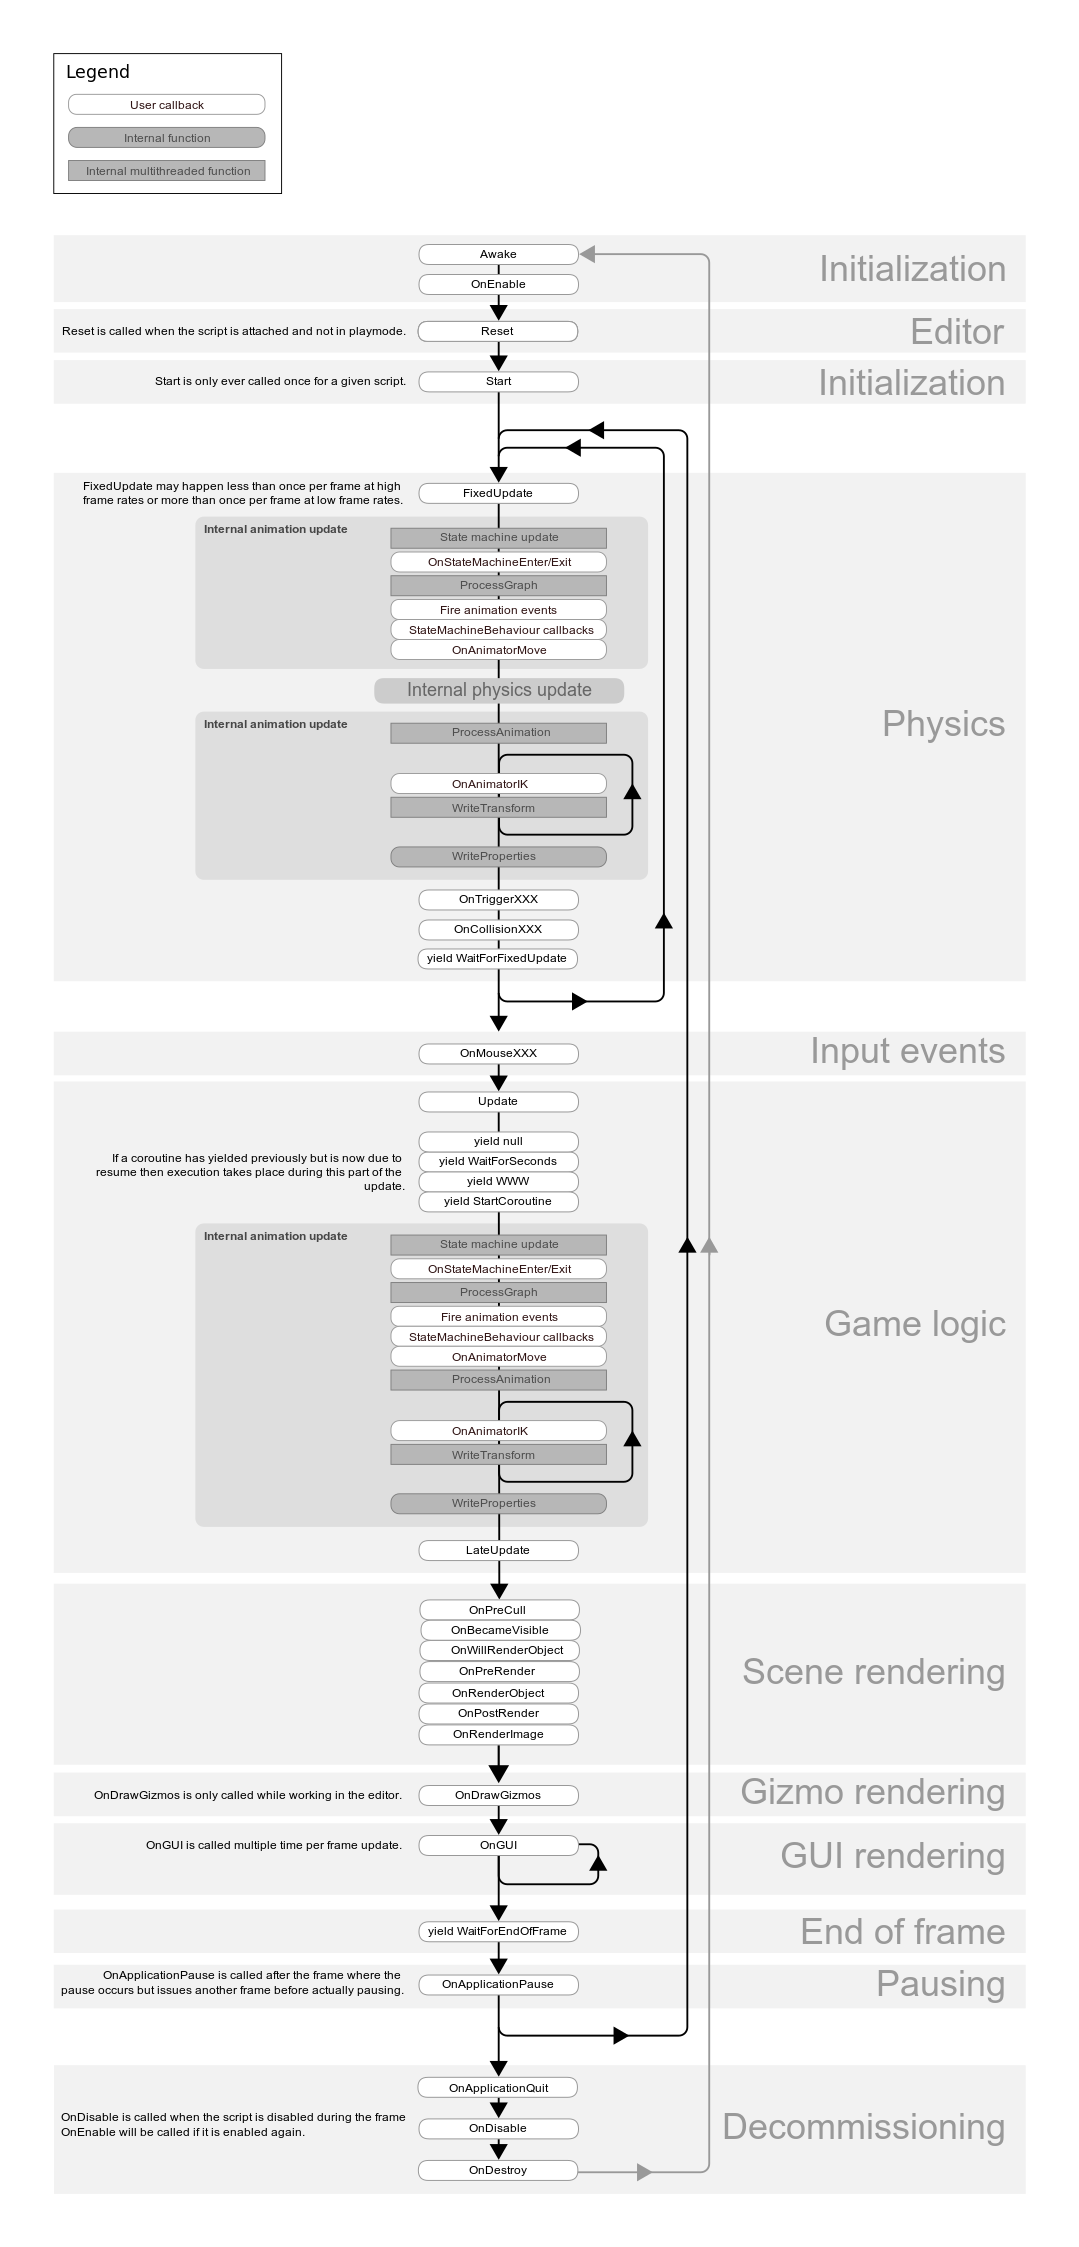
\includegraphics[width=10.5cm]{figures/UnityFlowchart.png}
    \caption{Unity Flowchart\cite{Unity:Flowchart}}
    \label{Unity:FlowchartFIG}
\end{figure}
\clearpage
Na rysunku\ref{Fig:UnityInterface} przedstawiono interfejs silnika unity.
Domyślnie jest on podzielony na 4 obszary. Pierwszy obszar znajdujący się w
lewej górnej części zawiera hierarchię obiektów na scenie. Na środku znajduje
się podgląd sceny. W prawej części znajduje się inspektor, który pozwala na
edytowanie pól obiektów znajdujących się na scenie. W dolnej części znajduje się
obszar zarządzania plikami oraz zakładka konsoli, w której wypisywane są błędy
oraz ostrzeżenia generowane przez edytor.

\begin{figure}[H]
    \centering
    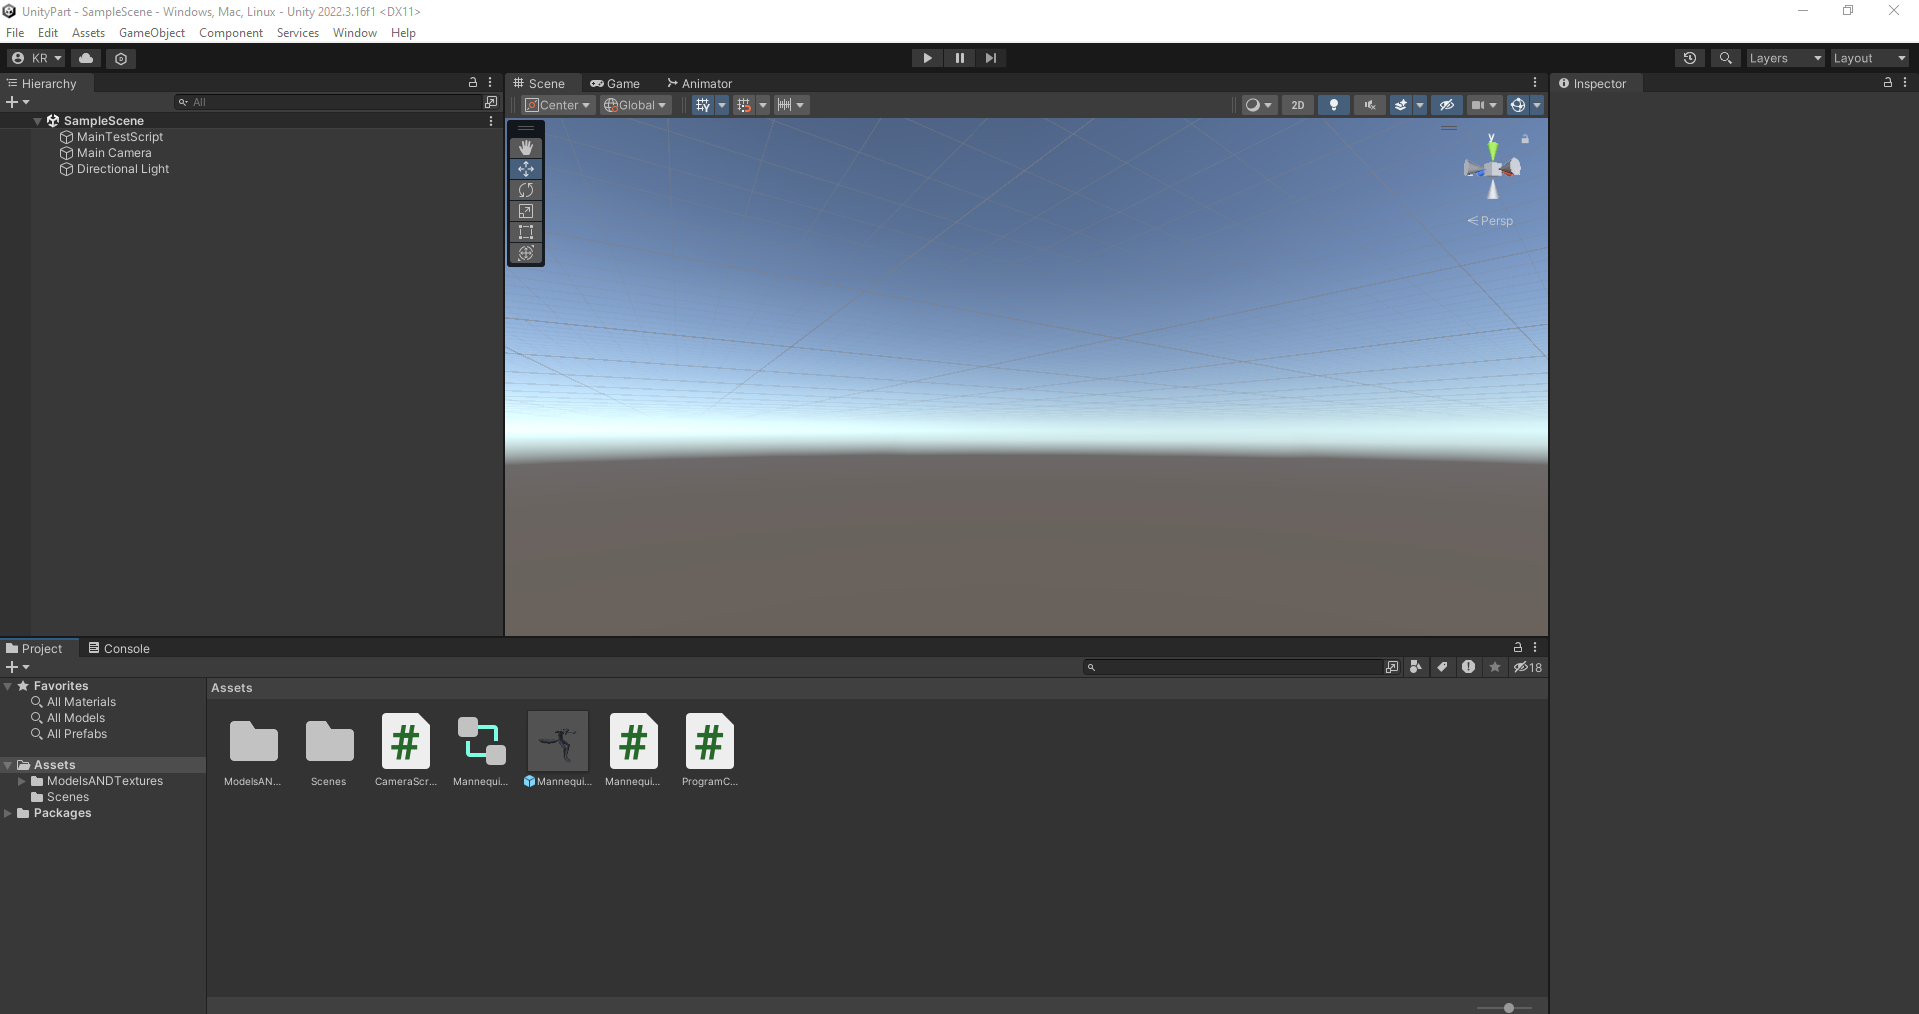
\includegraphics[width=16cm]{figures/InterfejsUnity.png}
    \caption{Wygląd interfejsu Unity}
    \label{Fig:UnityInterface}
\end{figure}  


\subsection{Architektura silnika Unreal Engine}
Do opisania silnika Unreal Engine wykorzystano dokumentację silnika \cite{UE:Documentatnion}.
Silnik Unreal Engine jest powstałym w 1991 roku rozwijanym do dzisiaj. Silnik
aktualnie jest jednym z najbardziej rozwiniętych silników graficznych. W silniku
można pisać kod na dwa sposoby: 
\begin{itemize}
\item Kod C++ -- Unreal Engine posiada możliwość pisania kodu za pomocą języka
C++. W tym przypadku twórca może tworzyć własne klasy za pomocą dziedziczeniu z
klas zaimplementowanych w silniku. Gry tworzone w ten sposób będą działać
szybciej niż te napisane za pomocą „Blueprint`ów” kosztem dłuższego czasu
kompilacji; 
\item Blueprint`y -- jest to programowanie obiektowe za pomocą bloków.
Programowanie w ten sposób działa podobnie do programowania za pomocą C++ -- jest
obsługiwane tworzenie programistycznych interfejsów, dziedziczenie i
przysłanianie metod. Zaletą tego rozwiązania jest szybkikrótki czas kompilacji.
\end{itemize}

Twórcy silnika Unreal Engine nie narzucają w jaki sposób należy używać ich
narzędzia. Obie metody programowania są ze sobą kompatybilne i można ich używać
naprzemiennie. Cały silnik jest bardzo plastyczny i jasno podzielony na wiele
klas, które można nadpisać\cite{UnrealEngineArchitecture}. 

Silnik został podzielony na 4470 różnych klas, które można nadpisać i dowolnie
używać, ale najczęściej używane to:
\begin{itemize}
\item GameInstance –- Istnieje tylko jedna instancja tej klasy w całym silniku,
która działa od rozpoczęcia programu do jego wyłączenia. Obiekt klasy może być
użyty w celu przechowywania danych między poziomami, zapisywania i wczytywania
danych np. zapisu gry lub ustawień gracza oraz do przechowywania funkcji, które
muszą być dostępne globalnie\cite{UE:GameInstance}; 

\item GameMode –- Klasa, która definiuje logikę w danym trybie gry. W grze może
być zaimplementowanych wiele trybów, ale tylko jeden obiekt typu GameMode może
istnieć. Obiekt tej klasy jest zawarty w obiekcie GameInstance. GameMode jest
odpowiedzialny za obsługę wejścia, kolizji oraz zmian poziomów, stworzenie
obiektu gracza i systemy zarządzania punktami. Zwykle każdy poziom ma swój
obiekt typu GameMode\cite{UE:GameModeState};

\item GameState –- klasa używana do przechowywania i zarządzania danymi pokroju
obecne punkty, pozostały czas, zdrowie gracza i inne ważne dane gry. Obiekt jest
zwykle zarządzany przez obiekt GameMode i w przypadku gry sieciowej jest
replikowany z serwera do klientów. Obiekt tej klasy jest łatwo dostępny przez
inne obiekty w programie pokroju kontrolerów gracza i obiektów klasy Actor.
Najważniejszą funkcją obiektów tej klasy jest synchronizacja stanu gry dla
wszystkich graczy\cite{UE:GameModeState};

\item Level Blueprint/LevelScriptActor –- specjalny typ aktora w silniku, który
pozwala na stworzenie logiki, która będzie wykonywana w czasie ładowania
poziomu. Obiekt klasy pozwala na ustawienie początkowego ustawienia klasy
GameState, stworzenie i ustawienie obiektów, aktywacja wydarzeń i wiele innych.
Klasa jest nadpisywana w celu stworzenia skryptów, które będą używane w
zależności od poziomu\cite{UE:LevelScriptActor};

\item Controller –- kontrolery dzielą się na dwie kategorie: kontrolery AI i
kontrolery gracza. Te obiekty tej klasy są odpowiedzialne za przetwarzanie i
przekazanie sygnałów wejścia do kontrolowanego obietku. Kontorlery determinują
sposób nawigacji postaci przez poziom, reakcję postaci w różnych sytuacjach oraz
interakcje z innymi obiektami w poziomie\cite{UE:Controller};


\item Pawn/Actor/Chracter -- Actor jest najbardziej podstawowym obiektem, który
można postawić na poziomie. W obiekcie tego typu znajdują się różne komponenty
typu oświetlenie, siatka czy kamera. Obiekty tego typu są bardzo proste i mogą
zostać użyte do implementacji własnych zachowań. Pawn jest klasą pochodną, która
posiada implementację złożonej fizyki, może oddziaływać na obiekty. Obiekty typu
Pawn są używane do stworzenia zachowań imitujących pojazdy lub zwierzęta.
Character jest klasą dziedziczącą z klasy Pawn. Obiekty klasy character w
porównaniu do dwóch poprzednich klas posiadają własną implementację ruchu,
komponentów animacji i zmiany wejścia na ruch fizyczny. Character jest klasą
używaną do stworzenia obiektu imitującego człowieka lub zwierzę z gotową
implementacją podstawowych mechanik\cite{UE:Actor,UE:Pawn,UE:Character};

\item Komponenty –- komponentami w UnrealEngine są wszystkie klasy, które
dziedziczą z klasy UActorComponent, a jest ich ponad 400. Komponenty zwykle
odpowiadają za jedną funkcjonalność np. oświetlenie, kolizje, fizyka, kamera,
siatka itp.  W ten sposób w silniku został stworzony stopień modularności, który
pozwala na wysoką elastyczność i skalowalność projektu. Jeden komponent może
zostać użyty w wielu różnych klasach. Komponenty mogą zostać użyte tylko\\w
klasach dziedziczących z klasy Actor lub innych komponentach\cite{UE:Component}.


\end{itemize}

Kolejną rzeczą, która jest ważna w programowaniu gier jest kolejność wykonywania
kolejnych części programu. W silniku Unreal każdy element jest inny i twórca
gier ma możliwość zmiany każdej części silnika. Poza tym silnik posiada wiele
metod, które są wspólne dla wielu elementów. Rysunek \ref{UE:ActorLifeCycle}
przedstawia cykl życia obiektu\\w silniku UnrealEngine. Na rysunku przedstawione
różne ścieżki. Jeżeli Aktor musiał być wczytany, ponieważ był częścią mapy, to
cykl życia zaczyna się od punktu `LoadMap`. Funkcja ‘AddToWorld’ jest częścią
działania ‘LoadMap’. Kolejnym ważnym punktem na tej ścieżce jest metoda
`PostLoad`, która jest wywoływana po wczytaniu mapy. 

Kolejną metodą jest `RouteActorInitialize`, który odpowiada za inicjalizacje
ścieżki poruszania się obiektu po świecie jeżeli została ustalona. Następnie
znajdują się 3 metody wywoływane podczas inicjalizacji komponentu. Powodem
stworzenia tych metod jest problem używania komponentów przez inne komponenty. W
`PreInitializeComponents` powinno się inicjalizować zmienne, tworzyć komponenty
i zmieniać ustawienia komponentu, który wywołał tę metodę.
`InitializeComponents` najczęściej jest używany podczas uzyskiwania dostępu do
innych komponentów. Ta metoda jest używana do uzyskania dostępu do innych
komponentów, punkcie czasu są one zainicjalizowane, ale nie można uzyskać
dostępu do niektórych pól. ‘PostInitializeComponents’ jest wywoływana jako
ostatni etap inicjalizacji. W tym momencie komponent skończył inicjalizację i
twórca kodu może w tym momencie wczytywać dane z innych komponentów należących
do tego samego pionka lub aktora bez błędu związanego z nieistnieniem obiektu.
Kolejną ważną i często używaną metodą jest metoda `BeginPlay`, która jest
wywoływana przed pierwszą klatką, kiedy dany pionek został stworzony lub po
wczytaniu poziomu. Metoda nie zostanie wywołana, jeżeli gra jest zapauzowana.
Przed omówieniem metody `Tick` należy opisać drogę od ‘SpawnActor’ i
‘SpawnActorDeffered’. Obie te ścieżki są podobne i główna różnica polega na
odroczeniu stworzenia obiektu. `SpawnActor` zacznie tworzyć aktora w momencie
wywołania metody `SpawnActor`. `SpawnActorDeffered` rozpocznie tworzyć obiekt po
pewnym czasie lub przy spełnieniu pewnych warunków. Konstruktor obiektu z języka
C++ zostanie wywołany dopiero w bloku `ExecuteConstruction`. W między czasie
jest wywołana metoda `OnConstruction` i `PostConstruction`. Metoda
`OnActorSpawned` zostaje wywołana po zakończeniu tworzenia obiektu. 

Najczęściej używaną metodą, która jest wywoływana co klatkę jest metoda ‘Tick’
na rysunku \ref{UE:ActorLifeCycle}. Tę metodę posiada każdy komponent i pionek
oraz każdy z tych obiektów może mieć wiele metod typu tick zgodnie z
dokumentacją \cite{UE:TickingActor}. Dodatkowo według tej samej dokumentacji te
metody mogą być wywoływane w różnym punkcie obliczeń silnika. W dokumentacji
wyróżniono 6 grup, kiedy metoda `Tick` może zostać wywołana, ale nie wszystko
zostało udokumentowane. Opisane grupy to:

\begin{itemize}
    


\item TG\_PrePhysics – pierwsza grupa, najczęściej odpowiada za aktualizację
stanu obiektów, na które wpływa fizyka, ale nie zmienia położenia, prędkości i
przyśpieszenia obiektów. Najlepszy moment na zebranie sygnałów wejściowych\\i
przekazanie ich do komponentów zajmujących się ruchem;

\item TG\_DuringPhysics – wszystkie komponenty używające kolizji lub fizyki muszą
zostać zaktualizowane. Obiekty znajdujące się w tej grupie obliczają kolizje i
inne elementy fizyczne. Twórcy gier mogą zmienić ustawienia silnika aby animacje
były aktualizowane w tej grupie. Obiekty w tej grupie mogą być aktualizowane
kilka razy w ciągu jednej iteracji pętli ze względu na możliwość implementacji
symulacji fizyki w silniku; 

\item TG\_PostPhysics – domyślnie do tej grupy należą wszystkie komponenty
zajmujące się animacjami, elementy interfejsu użytkownika i elementy graficzne;

\item TG\_POostUpdateWork – do tej grupy powinny należeć obiekty, które wymagają
dużej ilości obliczeń lub nie są istotne z punktu widzenia działania gry.
Obiekty w tej grupie są aktualizowane rzadziej niż te w innych grupach, więc
jest to idealna grupa dla sztucznej itenligencji, która wymaga dużej ilości
obliczeń. 
\end{itemize}

Zakończenie cyklu życia aktora w silniku Unreal Engine może rozpocząć się\\w
kilku przypadkach:
\begin{itemize}
\item Wywołanie metody `Destroy` - ze względu na architekturę silnika,
programista go używający nie może zniszczyć obiektów dziedziczących z klas
komponentów lub klasy aktora nie mogą być zniszczone wywołaniem zwykłego
destruktora. Metoda `Destroy` najpierw bezpiecznie usunie obiekt z elementów
silnika,\\a następnie wywoła destruktor obiektu;
\item Czas życia Aktora się skończył – w trakcie działania gry tworzonych i
usuwanych jest wiele obiektów. W silniku zaimplementowano mechanizm, który
pozwala na usuwanie obiektów po jakimś czasie ustalonym przez twórcę gry. Czas
życia obiektu można ustawić za pomocą metody ‘SetLifeSpan(float time)’, która
rozpocznie niszczenie obiektu po czasie podanym w sekundach;
\item Zmiana poziomu – gry mogą się składać z wielu poziomów i zabezpieczenie
programu przed wyciekami pamięci przy zmianie poziomów jest bardzo ważną rzeczą.
Przy zmianie poziomów wszystkie obiekty w poziomie zostają zniszczone i zostaje
wczytany nowy poziom; 
\item Zakończenie gry w Edytorze – testowanie funkcji w edytorze jest ważnym
elementem tworzenia elementów gry w każdym silniku. Gra w edytorze może być
włączana nawet kilkaset razy, co bez usuwania obiektów może doprowadzić do
wycieku pamięci i w konsekwencji wyłączenie się edytora;
\item Zakończenie gry – wywołane w przypadku zakończenia rundy, utraty
połączenia lub w przypadku osiągnięcia końca gry i wyświetlenia napisów
końcowych. 
\item Zakończenie programu.
\end{itemize}

Jeżeli jeden z tych warunków zostanie spełniony zostanie wywołana metoda
`EndPlay`. Metoda ma na celu zatrzymanie obiektu, zatrzymanie wywoływania metod
typu `Tick`, wysłanie sygnału o usuwaniu obiektu do obiektów `GameState`i innych
obiektów w grze. Obiekt zostanie oznaczony flagą `RI\_PendingKill`, co
zakolejkuje go do usunięcia za pomocą mechanizmu `Garabage Collector`. Przy
usuwaniu zostaną wywołane metody `BeginDestroy`, `IsReadyForFInishDestroy` i
`Finishdestroy`, w których powinna być zawarta implementacja usuwania elementów
alokowanych dynamicznie.  


\begin{figure}[ht]
    \centering
    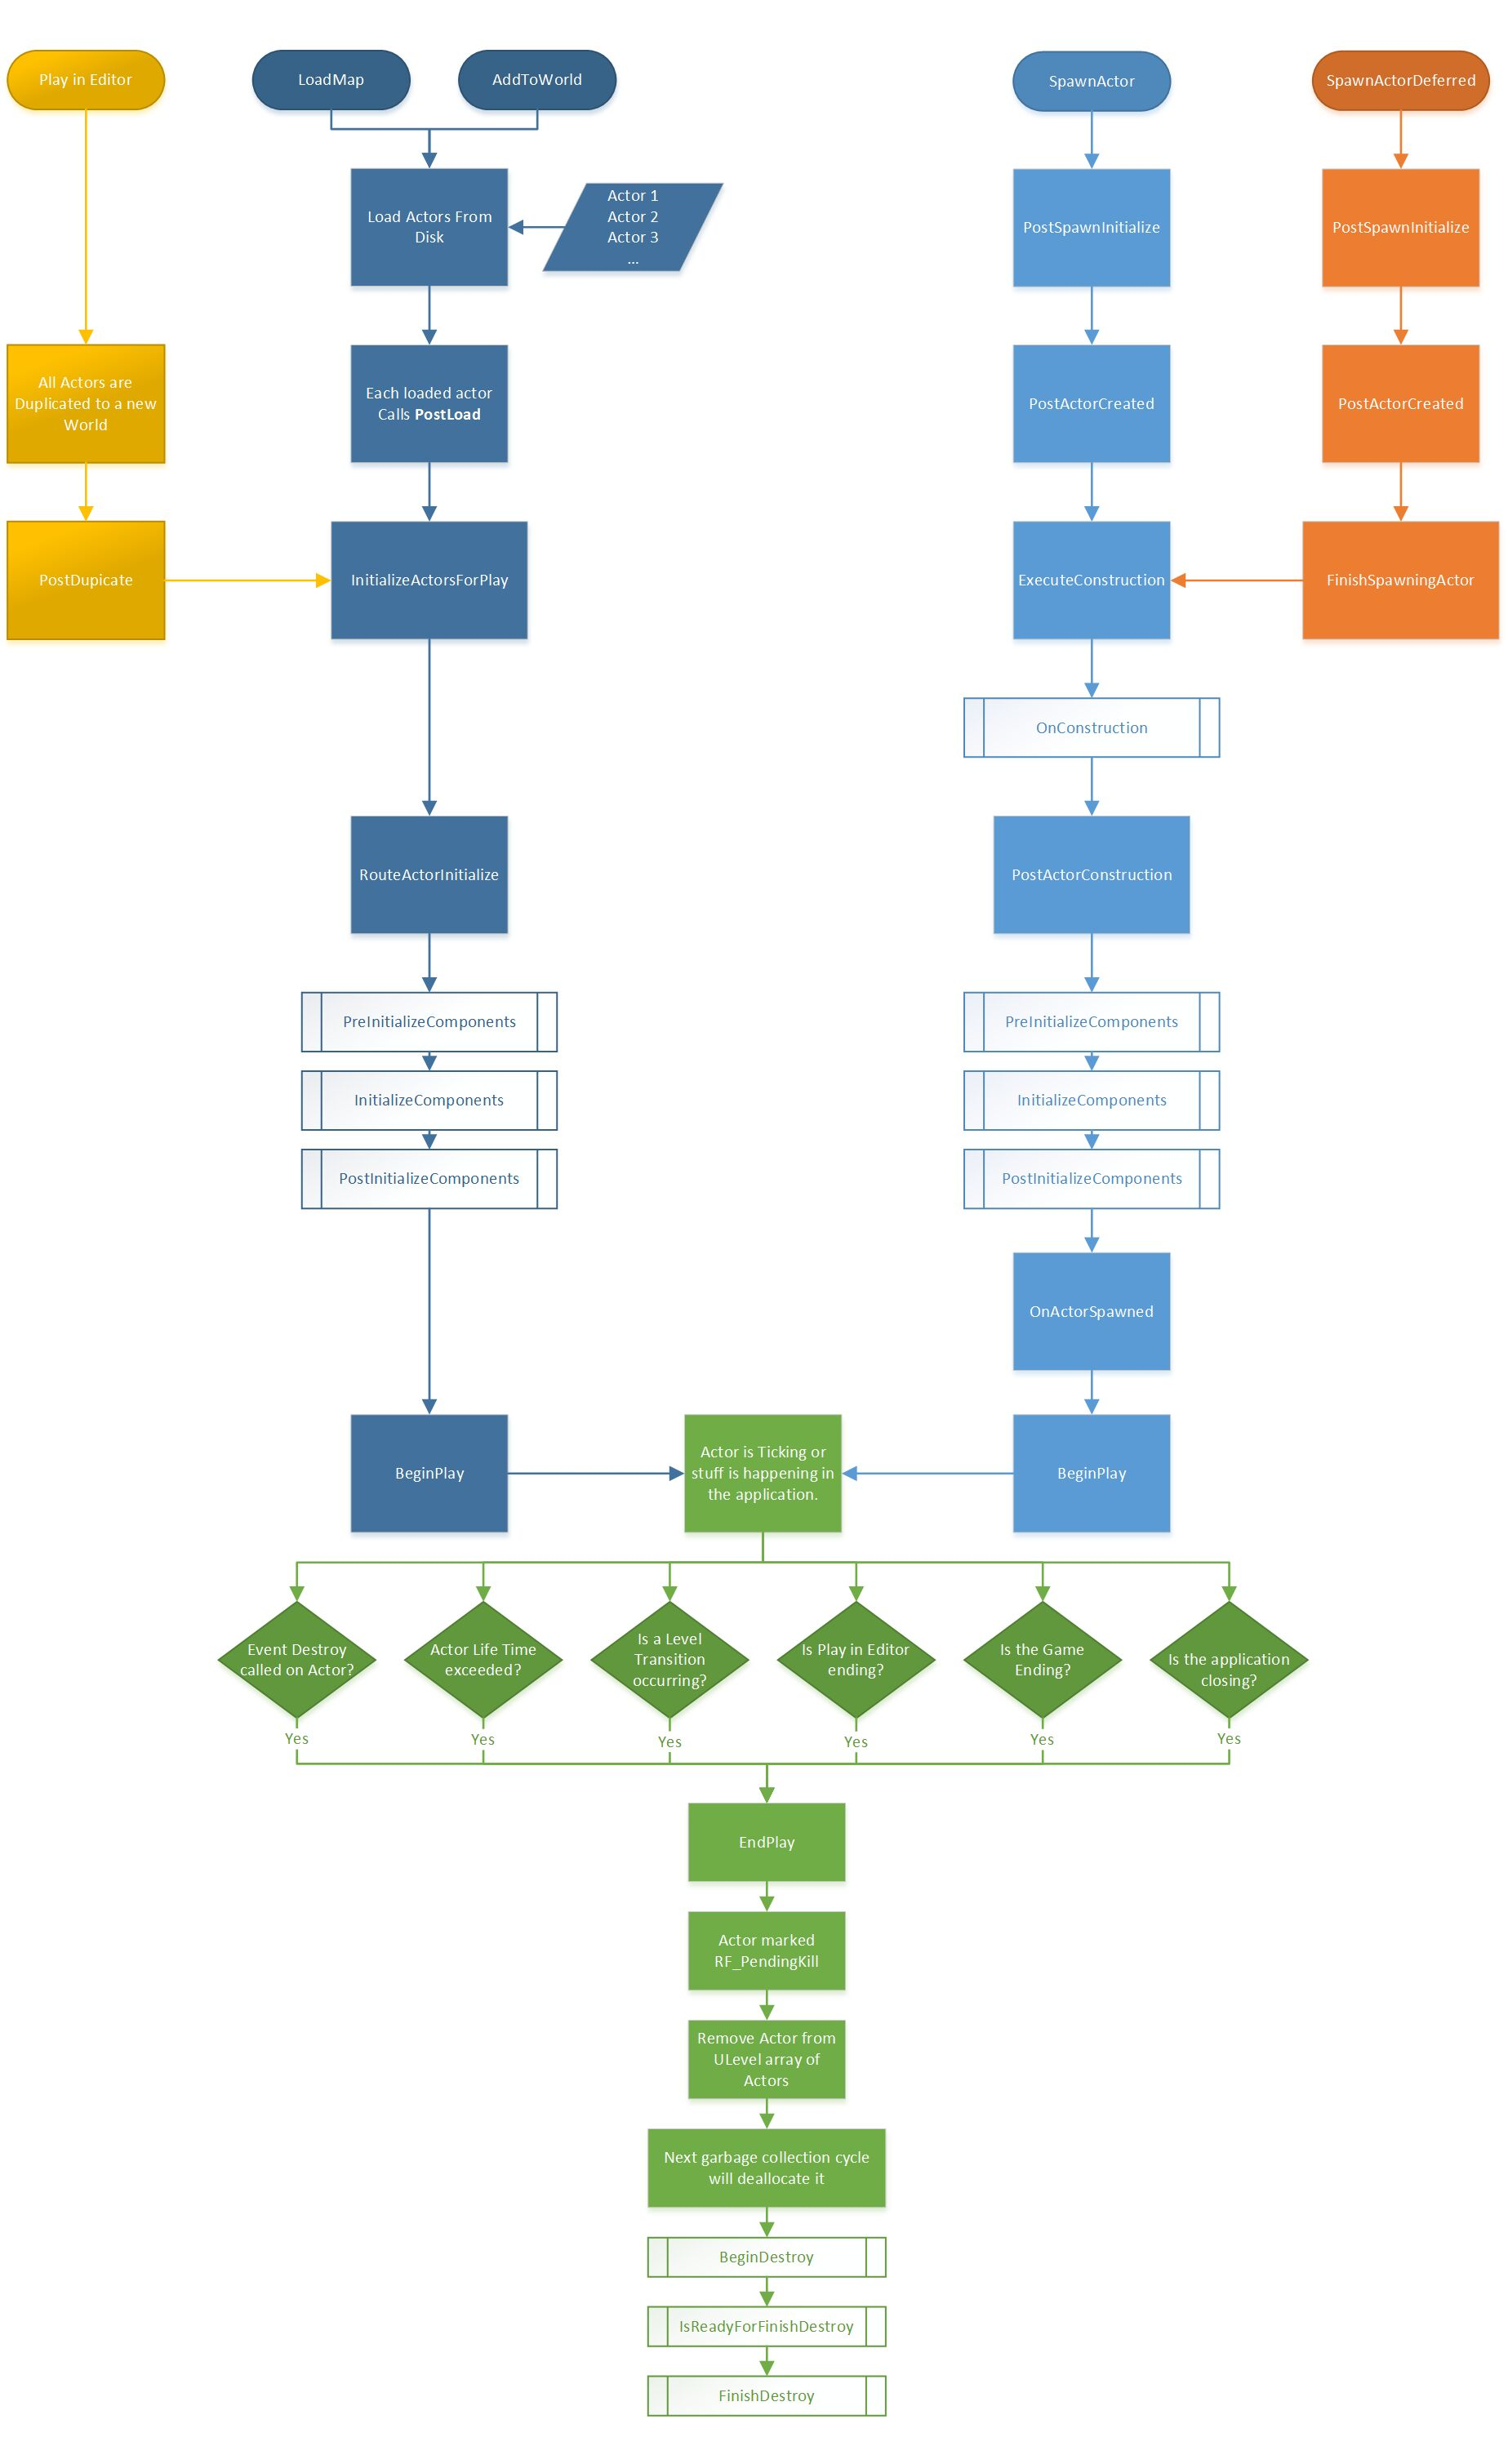
\includegraphics[width=14cm]{figures/ActorLifeCycle1UNREAL.jpg}
    \caption{Cykl życia obiektu w silniku Unreal Engine\cite{UE:ActorLifeCycleSource}}
    \label{UE:ActorLifeCycle}
\end{figure}
\clearpage
Na rysuniku \ref{UE:Intefrface} przedstawiono wygląd edytora silnika Unreal Engine.  Na
środku znajduje się podgląd poziomu. W podglądzie poziomu znajdują się różne
narzędzia np. perspektywy, skali okna, ustawień graficznych edytora oraz
narzędzia do edycji położenia obiektów. Po prawej stronie znajduje się narzędzie
zawierające listę aktorów w poziomie oraz okno, w którym można edytować pola
obiektów. W dolnej części znajdują się zakładki do przeglądania zawartości
projektu, konsola log’ów oraz konsola do komend silnika. 

\begin{figure}[ht]
    \centering
    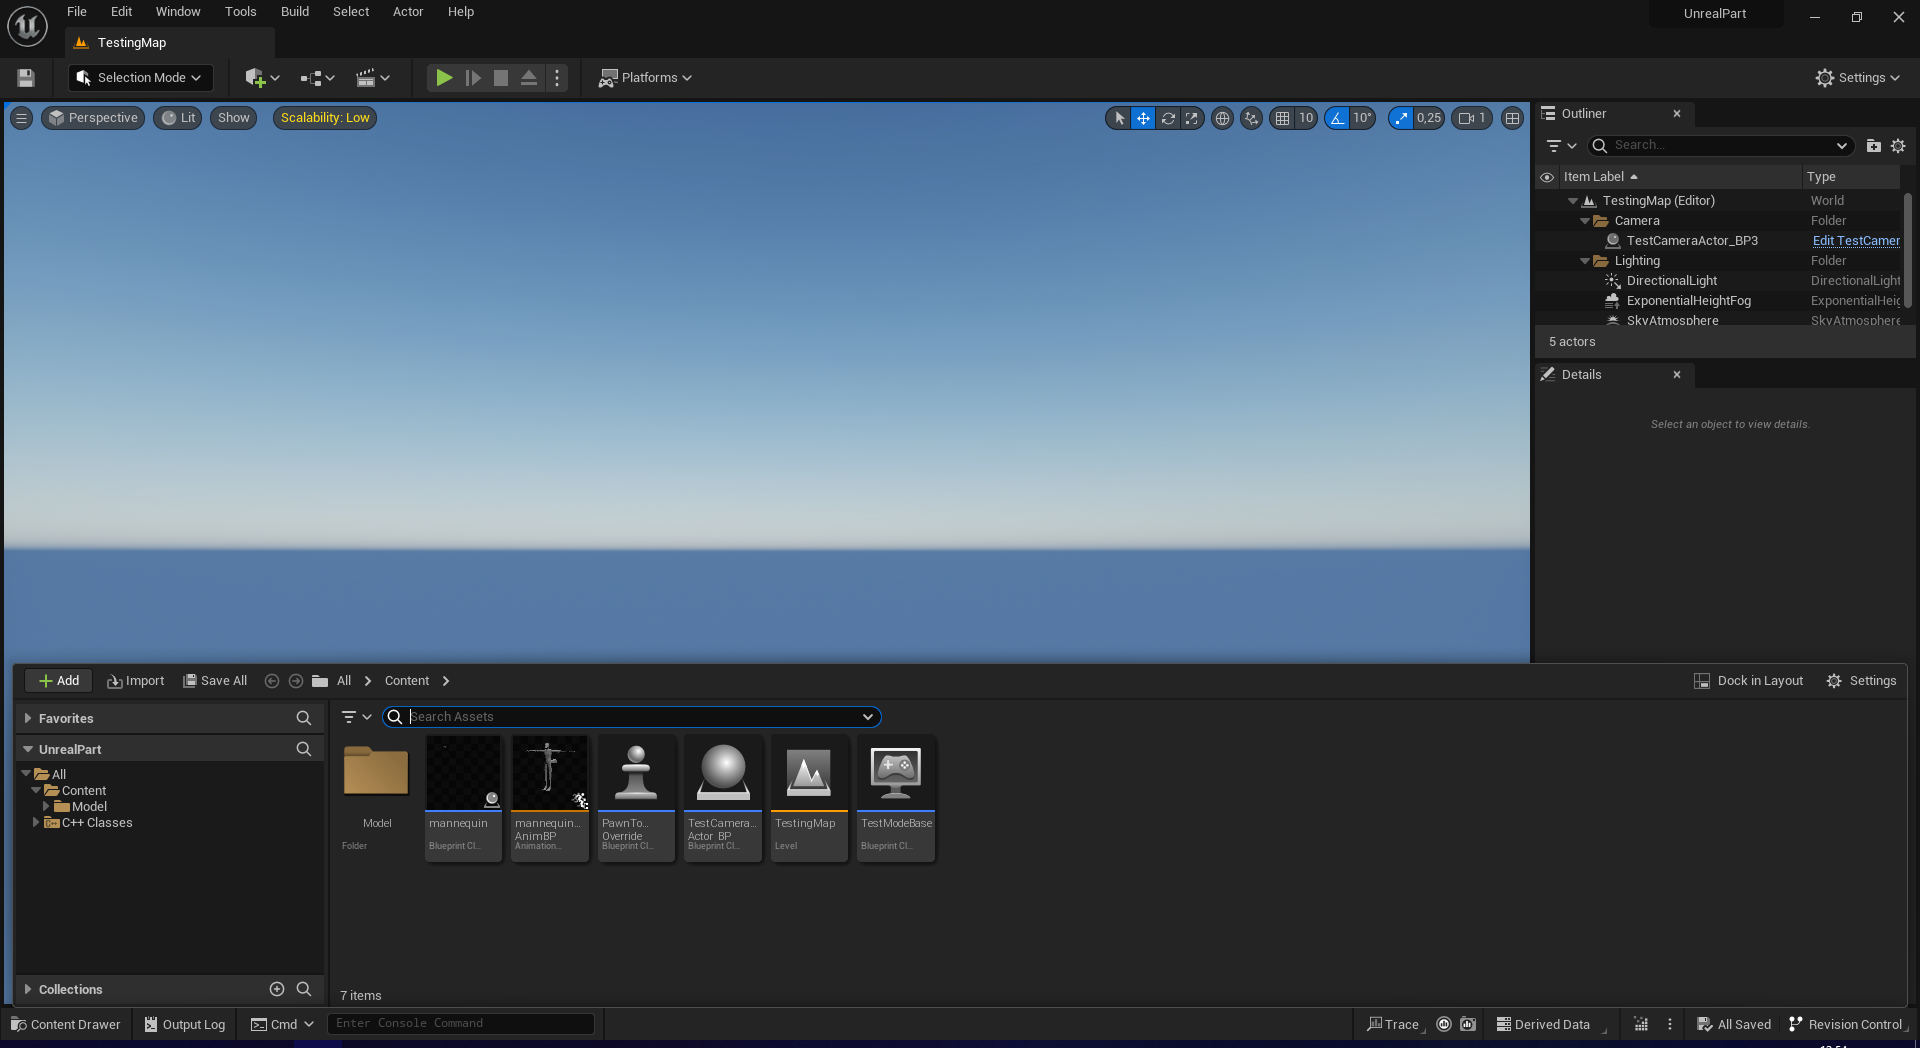
\includegraphics[width=14cm]{figures/InterfejsUnreal.png}
    \caption{Interfejs silnika Unreal}
    \label{UE:Intefrface}
\end{figure}

\subsection{Różnice między silnikami}


Poprzednie podrozdziały pokazały różnice w budowie i funkcjonowaniu silników.
Poza tym należy uwzględnić inne różnice między silnikami, które nie dotyczą ich
budowy, ale są ważnym elementem podczas programowania w obu silnikach. 

W tabeli \ref{Tabela:RozniceMiedzySIlnikami} przedstawia różnice między
silnikami, które można zauważyć przy korzystaniu z obu silników w dłuższym
okresie czasu. Pierwszą różnicą rzucającą się\\w oczy jest podstawowa jednostka
długości. W przypadku Unity jednostką odległości jest metr. W przypadku
prędkości jest to metr na sekundę. W Unreal Engine jednostką odległości jest
centymetr, a prędkości centymetr na sekundę. Z widzenia programisty jest to
ważna różnica, ponieważ wymagana jest konwersja jednostek w przypadku
korzystania ze stałych lub wzorów. Kolejną ważną różnicą jest oznaczenie osi,
która opisuje wysokość. W Unity wysokość jest oznaczona osią Y. Jest to ważne z
punktu widzenia programisty ponieważ domyślnie grawitacja jest skierowana
prostopadle w dół do osi oznaczającej wysokość. W Unreal Engine wysokość jest
opisana osią Z. 

Następnym punktem w tabeli są wbudowane elementy w silnik, które pozwalają na
zbudowanie gry. Unity posiada podstawowe funkcjonalności związane z animacjami i
ich edytowaniem, obsługą dźwięku, modeli, skryptów itp. Jest to jednocześnie
wada i zaleta silnika. Mała liczba gotowych elementów zmusza programistę do tworzenia
brakujących elementów lub korzystania z elementów stworzonych przez społeczność.
Takie podejście jest jednak czasochłonne i może doprowadzić do błędów w
działaniu gry. Unreal Engine stoi po przeciwnej stronie medalu. Silnik zapewnia
wiele elementów, stworzonych przez twórców silnika, które zostały przetestowane
i sprawdzone, jednak takie podejście ogranicza w pewnym stopniu kreatywność. 

Kolejnym punktem zapisanym w tabeli \ref{Tabela:RozniceMiedzySIlnikami} jest
podział skryptów. W Unity wszystko zostało zawarte w ‘Monobehaviour’. Unreal
Engine każdą klasę posiada\\w osobnych plikach z rozszerzeniami ‘.h’ i ‘.cpp’, co
jest standardem w przypadku programowania obiektowego w języku ‘C$++$’. Wadą
tego rozwiązania jest szukanie pewnych klas i funkcji oraz długi czas kompilacji
projektu. Rozwiązaniem problemu jest użycie ‘Blueprintów’ razem z
‘C$++$’.’Blueprinty’ pozwalają na szybkie prototypowanie, jednak kod zapisany w
ten sposób jest wolniejszy niż ten zapisany w ‘C$++$’.


Budowa silników została opisana w poprzednich rozdziałach. Unity ma prostą
budowę składającą się z 3 elementów. Zaletą tego rozwiązania jest lekkość
silnika,\\a wadą brak rozwiniętej infrastruktury gry. Unreal Engine posiada
bardziej rozwiniętą infrastrukturę, ale przez to wymaga więcej wiedzy na temat
silnika oraz języka programowania w celu wykorzystania w pełni tej cechy
silnika.

 



\begin{table}[ht]
\caption{Znaczące różnice między silnikami Unity i Unreal Engine}
\centering		
	\begin{tabular}{|p{3cm}|p{5,5cm}|p{5,5cm}|}	
		\hline
		Różnica & Unity & Unreal Engine  \\
		\hline
		Podstawowa jednostka długości & metr & centymetr \\
		\hline
		Oznaczenie osi & Y oznacza wysokość & Z oznacza wysokość \\
		\hline
		Wbudowane funkcjonalności & Wymaga zbudowania gry od podstaw lub
		używania plugin’ów & Posiada wbudowane funkcje, które występują w wielu
		grach \\
		\hline
        Podział skryptów & Wszystko zawarte w Monobehaviour & Wszystkie
        są zapisane w osobnych plikach \\
        \hline
        Podział elementów silnika & Scena, Obiekt, Komponent & Instancja
        silnika, GameMode, GameState, Level, Controller, Aktor, Komponent \\
        \hline
	\end{tabular}	
	
\label{Tabela:RozniceMiedzySIlnikami}
\end{table}	






\clearpage	
\section{Porównanie wydajności silników Unity i Unreal Engine}

%\subsection{Założenia, zakres testów oraz klasyfikacja danych}

Głównym testem jest sprawdzenie jak silniki radzą sobie z generacją obrazu\\w
czasie rzeczywistym. Obiekty są prostymi modelami z zapętlonymi animacjami
wybranymi wcześniej w sposób losowy – rozstawienie, animacje i prędkość animacji
zostaną wygenerowane skryptem i były takie same dla obu silników. Modelem i
animacjami użytymi w testach były te, które zostały wykonane w projekcie
inżynierskim \cite{ModelSource}. Na scenie zostanie wielokrotnie rozmieszczony
autorski model postaci z wcześniej opracowanej gry wykonujący pewne animacje
szkieletowe. Autor wyraził zgodę na użycie modelu w pracy.


Silniki graficzne są bardzo złożone, dlatego test obejmuje tylko jeden aspekt
jakim jest renderowanie dynamicznie rozstawionych obiektów wraz z animacjami.
Obiekty w świcie gry mogą być statyczne, co oznacza, że nie można ich ruszyć i
nie działają na nie prawa fizyki. Silniki graficzne mogą zmniejszać wymagania
obliczeniowe związane\\z tym obiektem przykładowo poprzez wypalania oświetlenia.
Dynamicznymi obiektami są określane wszystkie obiekty, które można
przemieszczać, poruszają się same z siebie albo są zaanimowane. 

Gry komputerowe trafiają na różne urządzenie z różną mocą obliczeniową.
Dodatkowo komputery posiadają wiele programów i usług działających w tle, które
mają wpływ na wynik testów. Te czynniki należy wziąć pod uwagę podczas trwania
testów. Dlatego testy odbędą się na komputerach stacjonarnych i laptopach z
systemem Windows 10 i Windows 11. System operacyjny został wybrany ze względu na popularność
wśród graczy. Zgodnie z badaniem z lutego 2024 roku wykonanym przez platformę
Steam\cite{SteamSurvey}, która jest największa aplikacją sprzedająca gry na komputery. Gracz
korzystający ze sklepu najczęściej używają systemów Windows 10 i Windows 11
stanowiących odpowiednio 53,19\% i 41,96\% wszystkich graczy co zosstało
przedstawione na rysunku
\ref{SteamHardwareSoftwareSurvay}. W badaniu również znalazły się dane na temat
używania poszczególnych komponentów przez graczy. Można odczytać, że gracz
najczęściej posiadają 16GB pamięci ram i ta grupa stanowi prawie połowę
wszystkich graczy. Procesory graczy pracują w taktowaniu od 2.3 do 2.69GHz.
Największa różnorodność można dopatrzyć się w używanych kartach graficznych.
Najczęściej używaną kartą graficzną jest karta GeFroceRTX 3060, której używa
6\% graczy. Ponad połowa graczy używa rozdzielczości 1920x1080. Jedna trzecia
graczy posiada w swoich kartach graficznych 8GB pamięci VRAM.

\begin{figure}[H]
    \centering
    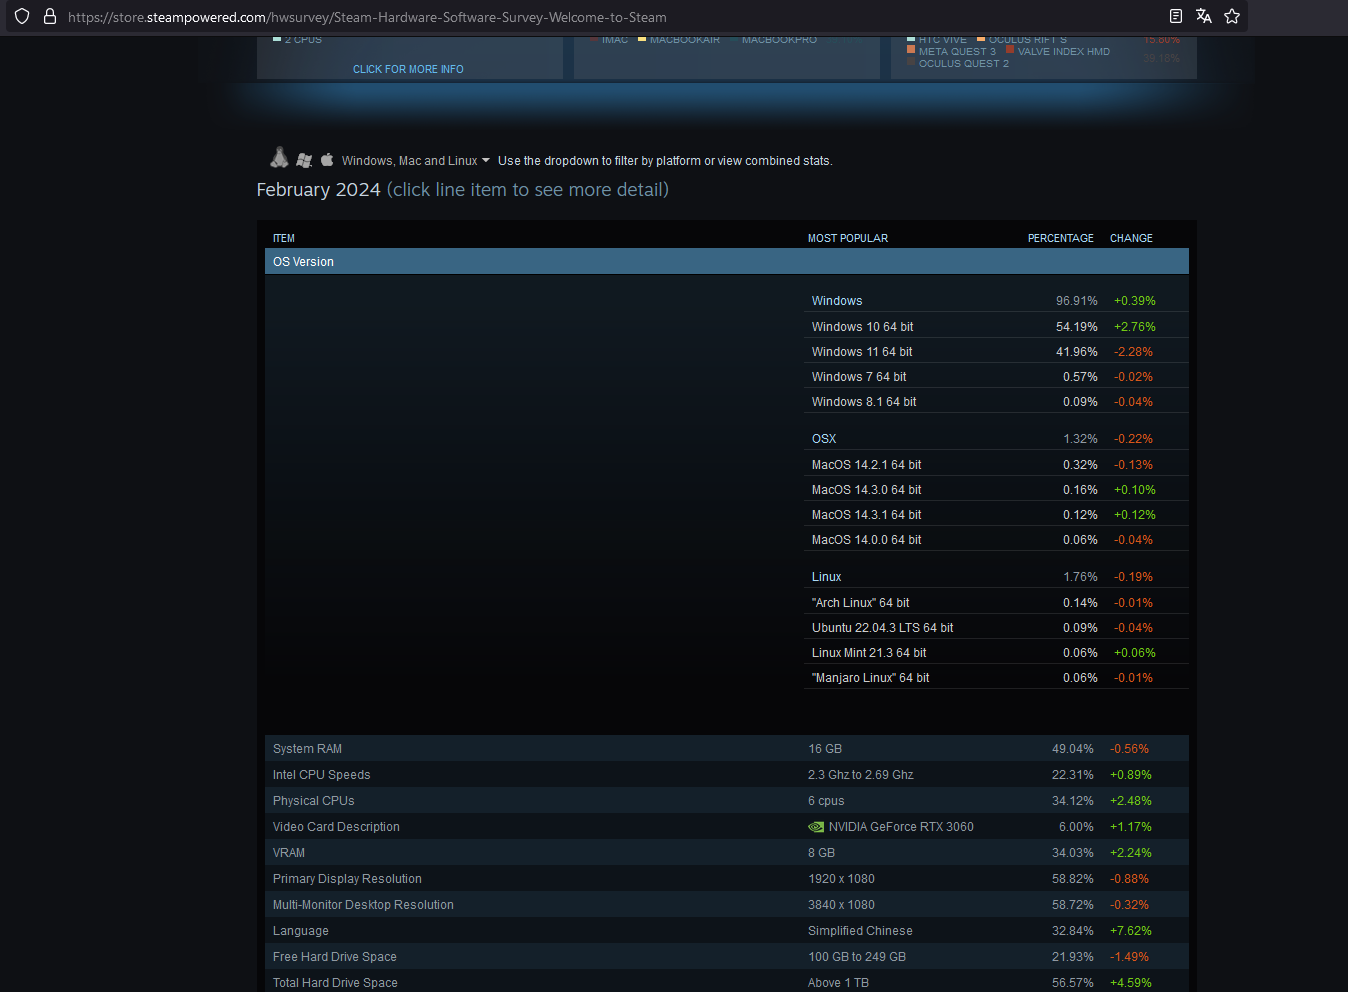
\includegraphics[width=14cm]{figures/SteamHardwareSoftwareSurvay.png}
    \caption{Statystyka użycia systemów operacyjnych przez graczy komputerowych przeprowadzona przez Steam \cite{SteamSurvey}}
    \label{SteamHardwareSoftwareSurvay}
\end{figure}



Głównym celem testów jest oszacowanie, który silnik graficzny lepiej radzi sobie
z generacją klatek w czasie rzeczywistym. Kryteriami oceniania są:

\begin{itemize}
\item Licznik FPS – jest to wartość równa 1/(czas wykonania programu między
klatkami). Różnica między 1-2 klatkami na sekundę nie jest znacząca. Dodatkowo
można określić stabilność na podstawie różnych miar pokroju minimum, maskimum i
odchylenie standardowe. Dodatkowo zostały opracowane wykresy pokazujące
wyświetlaną liczbę klatek w danej sekundzie testów dla każdego komputera, na
którym dobył się test;   
\item Użycie czasów procesora i procesora graficznego – ważne kryterium, które
pomoże ustalić, która część komputera jest mocniej wykorzystywana podczas testu.
Zostało uzyskane średnie, minimalne i maksymalne użycie; 
\item Zużycie pamięci RAM i VRAM – Zużycie pamięci RAM i VRAM – ostatni
wyznacznik. Zbyt mała ilość pamięci RAM i VRAM może doprowadzić do
nieuruchomienia się gry.  Najważniejsza jest maksymalna ilość używanego zasobu
podczas testu, a średnie i minimalne użycie jest ciekawostką. Maksymalne
wartości pozwolą na określenie, który silnik lepiej gospodaruje zasobami. 
\end{itemize}

Do zbierania danych o użyciu procesora, pamięci RAM, pamięci VRAM karty
graficznej i procesora graficznego użyto wbudowanych narzędzi i bibliotek w
silniki. Powodem wybrania takiego rozwiązania jest uproszczenie uruchomiania
testów na wielu komputerach i eliminuje potrzebę instalacji zewnętrznego
oprogramowania. 


Liczba rozłożonych obiektów została dobrana metodą prób i błędów zaczynając od
20 tysięcy. Liczba była dobrana w taki sposób, aby prędkość wyświetlania klatek
na jednym z silników wynosiła co najmniej 15 klatek na sekundę, a na drugim
silniku było co najmniej 10 klatek na sekudnę w edytorze obu silników. Powodem
takiego kryterium było doprowadzenie do sytuacji, gdzie oba silniki będą
pracowały pod znacznym obciążeniem, co z kolei pozwoliło na zanotowanie
fluktuacji w szybkości wyświetlania kolejnych klatek. Jest to bardzo ważne z
perspektywy osoby używającej produkt końcowy, czyli graczy. Duże zmiany w
szybkości wyświetlania kolejnych klatek mogą zmienić odbiór gry. Pierwszym
krokiem stworzenia testu jest utworzenie projektu na obu silnikach. Zostały
wykorzystane ‘puste’ projekty oferowane przez oba silniki graficzne. Przez
domyślne ustawienia silników testy mogą wydawać się inne od siebie. Jest to
iluzja spowodowana innymi ustawieniami kamer w obu silnikach. Kamera w obu
silnikach porusza się za pomocą fizyki w grze. Dla kamer została wyłączona
grawitacja.  Kamery poruszają się ruchem jednostajnym prostoliniowym od punktu
do punktu na ścieżce. Po osiągnięciu punktu zostaje wczytany następny punkt, aż
do osiągnięcia ostatniego punktu, co spowoduje wyłącznie się testu. Po
osiągnięciu każdego następnego punktu kamera zmienia rotację. Kamera może być
ustawiona tak, aby patrzeć się w kierunku jakiegoś punktu. W końcowych fazach
testu kamera jest ‘teleportowana’ po czym przez krótki czas rusza się do przodu
ruchem jednostajnym. Ważne aby skrypty w silnikach działały w podobny sposób.
Projekty zostały zbudowane i testy zostały przeprowadzone na zbudowanych
projektach. 


\subsection{Przygotowanie testu Unity}

Do zbierania informacji o użyciu zasobów w trakcie testów z silnikiem Unity
został wykorzystany ‘Profiler’ silnika. Profiler jest narzędziem do określenia
ile zasobów wymagają pewne części gry. Narzędzie pozwala na twórcom gier na
podjęcie próby optymalizacji programu do takiego stopnia, aby gra działała
płynne na pewnej grupie urządzeń. W skrypcie narzędzia te znajdują się w
‘UnityEngine.Profiling’\\i ‘Unity.Profiling’. Narzędzie ma wadę, która nie
pozwala na zbieranie danych co klatkę, ale co pewien czas. W programie
wykorzystano następujące metody i klasy:
\begin{itemize}
\item Profiler.GetTotalReservedMemoryLong() – metoda zwraca ilość używanej
pamięci RAM podaną w bajtach; 
\item Profiler.GetAllocatedMemoryForGraphicsDriver() – metoda zwraca ilość
pamięci karty graficznej VRAM użytej przez program. Zwraca wartość podana jest w
bajtach; 
\item ProfilerRecorder – klasa używana do zliczania ile czasu pracował dany
podzespół komputera w określonym czasie. W programie testowym obiekty klasy
zostały użyte do zliczenia czasu pracowały procesor i karta graficzna. W
obiektach zapisywane są próbki. Czas pracy jest zapisany w nanosekundach. W
próbek została wyciągnięta średnia.
\end{itemize}
Dane z narzędzia w teście są zbierane co 0.5 sekundy. Liczba FPS była zbierana
co klatkę. Profiler jest słabo udokumentowanym narzędziem oraz wymaga zbudowania
programu w trybie developerskim.

W projekcie Unity na scenie istnieją tylko 3 obiekty i są nimi obiekt
rozstawiający modele, obiekt z komponentem kamery oraz obiekt\\z źródłem światła.
Obiekt\\z kamerą posiada odpowiedni skrypt, który wczytuje następne punkty drogie
i wyłącza program po dotarciu do ostatniego punktu. Obiekty imitujące model są
tworzone\\z ‘prefab’a’, w którym znajduje się model i animator do zarządzania
animacjami. Na rysunku \ref{Fig:UnityAnimation} pokazano jak wygląda maszyna
stanów aniamtora. Stanem wejściowym jest ‘InitState’, od którego są poprowadzone
przejścia do innych stanów animacji. Przejście między stanami jest zależne od
wartości parametru ‘AnimationID’. 



Na rysunku \ref{Fig:TESTUnityScreen} przedstawiono jak wyglądają pierwsze sekundy testu zbudowane na silniku Unity. 

\begin{figure}[h]
    \centering
    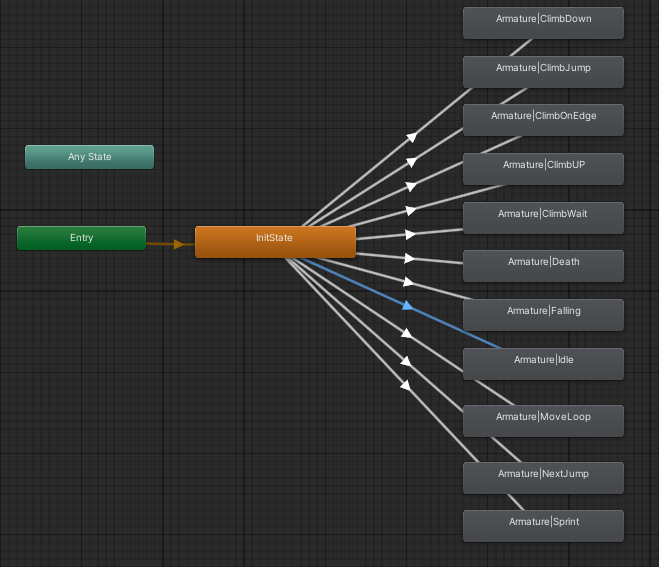
\includegraphics[width=16cm]{figures/UnityAnimation.png}
    \caption{Stany animacji w Animatorze w Unity}
    \label{Fig:UnityAnimation}
\end{figure}     
\clearpage
\begin{figure}[H]
    \centering
    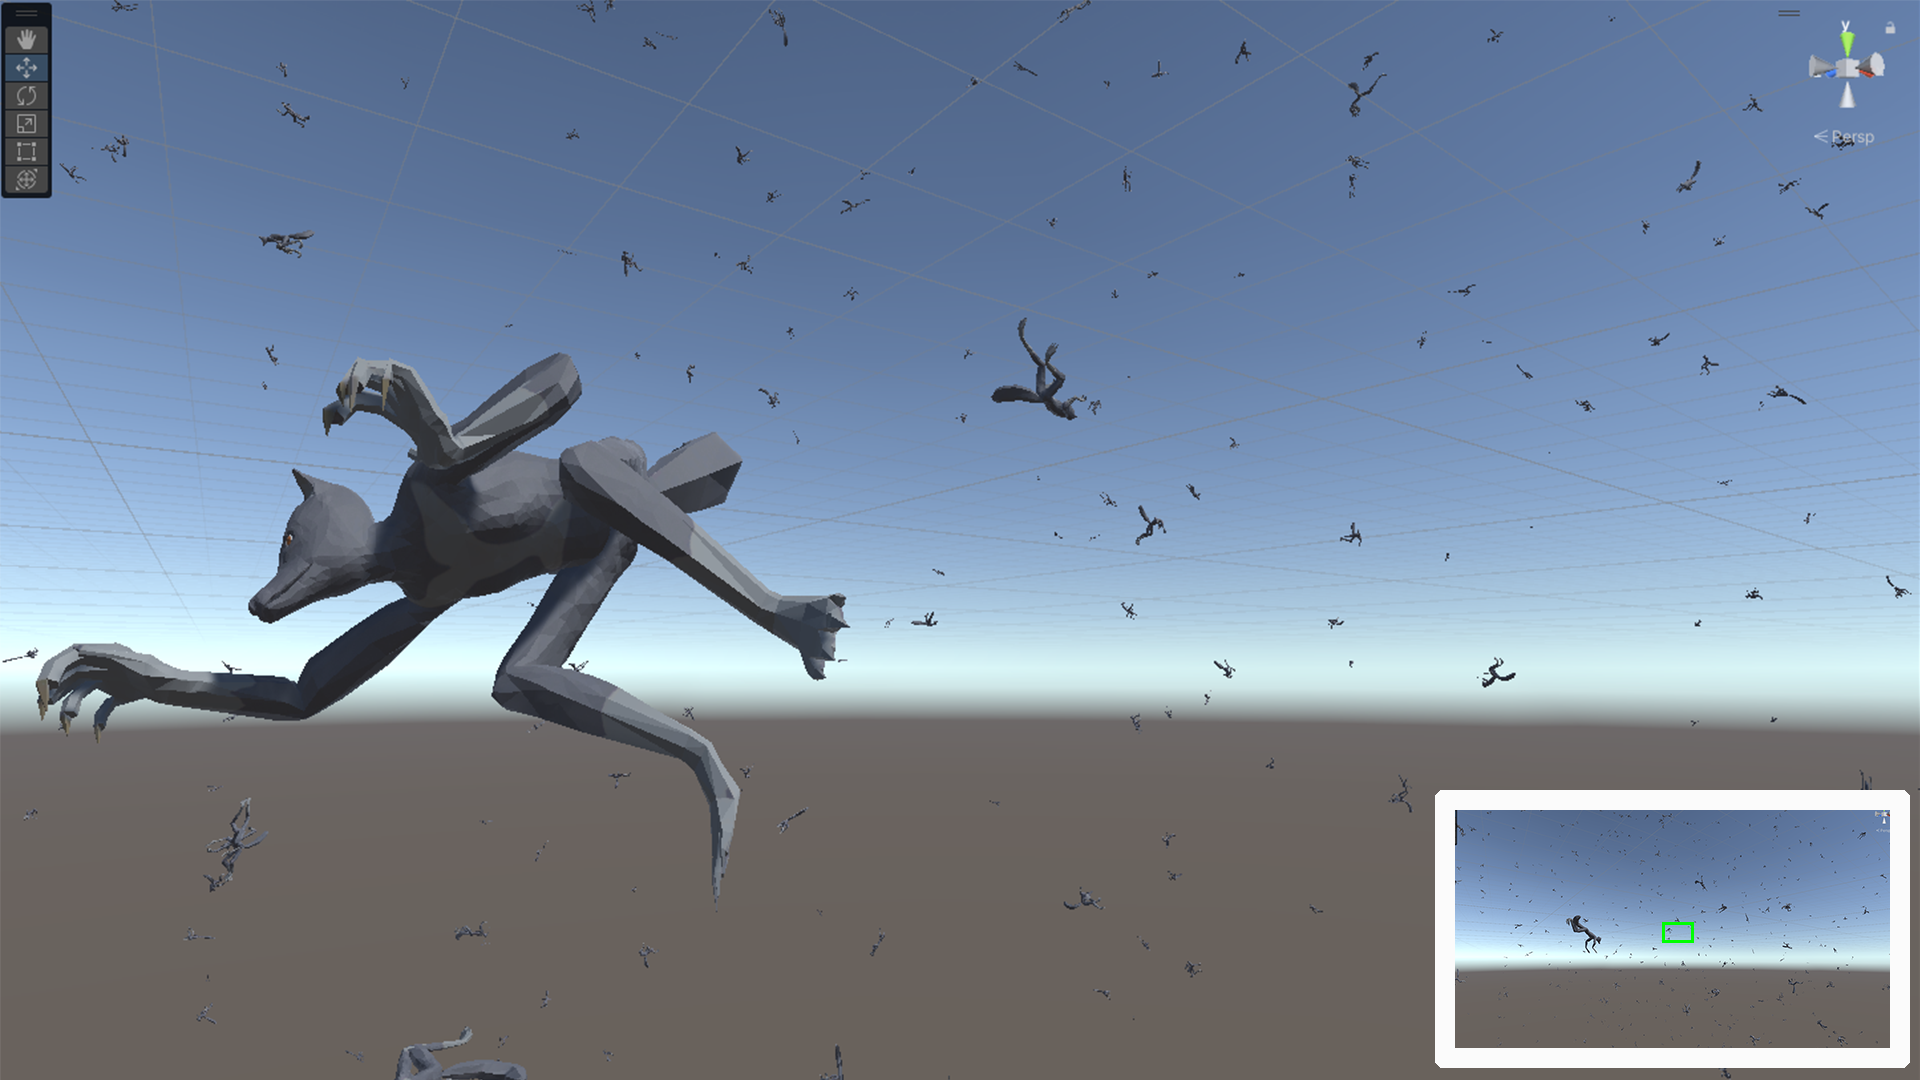
\includegraphics[width=16cm]{figures/UnityLupa.png}
    \caption{Wygląd testu silnika Unity w pierwszych sekundach }
    \label{Fig:TESTUnityScreen}
\end{figure}     


\subsection{Przygotowanie testu Unreal Engine}

W silniku Unreal Engine informacje o użyciu czasu procesora, pamięci RAM i pamięci karty graficznej są zapisywane w klasach rodziny ‘FPlatform’. Z tych klas wykorzystano następujące metody i pola:
\begin{itemize}
\item ‘GetPerFrameProcessorUsage’ jest metodą zawartą w klasie
‘FPlatformMemory’, która zwraca czas procesora użyty w danym procesie gry. Za
argumenty przyjmuje ID procesu i dwie referencje typu float. W tych referencjach
zostaną zapisane czas obliczeń procesora oraz czas oczekiwania procesora jako
procent czasu pracy. Suma tych wartości wskazuje jaką część całkowitego czasu
pracy procesora zastało poświęcone na grę. Czas oczekiwania procesora określa
jak długo procesor oczekiwał na dane z pamięci itp.;
\item Metoda GetStats z klasy FPlatformMemory pozwala na uzyskanie danych\\o
pamięci komputera. Metoda zwraca obiekt FPlatformMemoryStats, z którego pole
UsedPhysical zwraca ile pamięci RAM jest używane przez aplikację w poprzedniej
klatce podane w bajtach;
\item GGPUFrameTime jest polem, które przechowuje liczbę cykli procesora karty
graficznej użytych w poprzedniej klatce. Zamiast odwołania do pola można wywołać
metodę ‘FPlatformTime::Cycles()’.
\end{itemize}
Do uzyskania informacji o ilości użytej pamięci karty graficznej przez program
użyto biblioteki ‘RHI’. ‘RHI’ jest interfejsem pomiędzy kartą graficzną, a
programem. Z biblioteki została użyta metoda ‘GetUsedMemory’, która zwraca ilość
używanej pamięci karty graficznej w kilobajtach. Działanie ‘RHI’ nie wymaga
działania silnika w trybie developerskim. 

Obiektem używanym do rozstawienia modeli i zapisania danych o użytych zasobach
był obiekt poziomu stworzony na podstawie klasy dziedziczącej z
‘LevelScriptActor’. Wymagało to zmiany klasy bazowej w poziomie. Do zapisywania
danych wykorzystano bibliotekę standardową z języka C$++$, ponieważ były
prostrze w obsłudze te wbudowane w silnik Unreal Enigne. Zapisany poziom
należało ustawić jako domyślny w ustawieniach projektu. Podobnie należało
postąpić z domyślnym ‘pawn’em’, którego należało podmieć na innego, który będzie
sterował kamerą. Ten pionek posiada w sobie komponent kamery, który będzie
funkcjonował jako domyślna kamera w teście, gdy domyślny pionek zostanie
stworzony. ‘RootComponent’ jest ‘BoxComponent’, dzięki czemu pionek mógł się
ruszać za pomocą prostej fizyki. Do tego komponentu został podłączony komponent
kamery. Przy wczytywaniu następnych punktów w ścieżce kamery oraz prędkości
kamery należało pamiętać o konwersji jednostek. W miejsca, gdzie miały być
modele z animacjami zostali stworzeni aktorzy, którzy posiadali
‘SkeletalMeshComponent’. Ten komponent wymaga ustawienia klasy animacji. Klasa
animacji w projekcie nazwana ‘mannequinAnimBP’ jest ‘Blueprint’em’ dziedziczącym
z klasy ‘AnimIsntance’, co pozwoliło na ustawienie prostej maszyny stanów, która
pozwoliła na ustawienie zapętlonej animacji. 
Na rysunku \ref{Fig:UnrealManequin} przedstawiono drzewo przejść animacji.
Przejścia polegają na porównaniu zmiennej ‘AnimationIndex’ do ustawionej liczby
stałej. Węzeł ‘Temp’ jest domyślnym węzłem, z którego jest przejście do reszty
węzłów. 

Rysunek \ref{Fig:TESTUnrealScreenLUPA} przedstawia pierwsze kilka sekund testu.
Rozstawieni aktorzy odtwarzają wybraną animację zapętloną w nieskończoność. 



\begin{figure}[h]
    \centering
    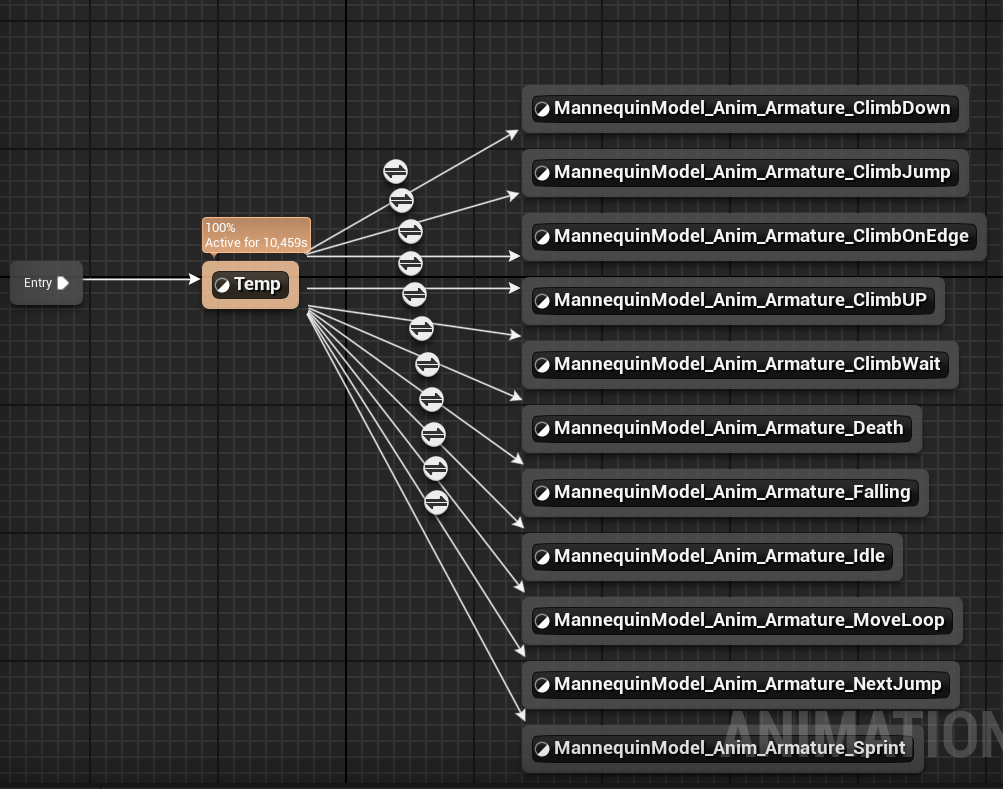
\includegraphics[width=16cm]{figures/UnrealManequin.png}
    \caption{Drzewo przejść animacji w silniku Unreal Engine}
    \label{Fig:UnrealManequin}
\end{figure}     

 


\begin{figure}[h]
    \centering
    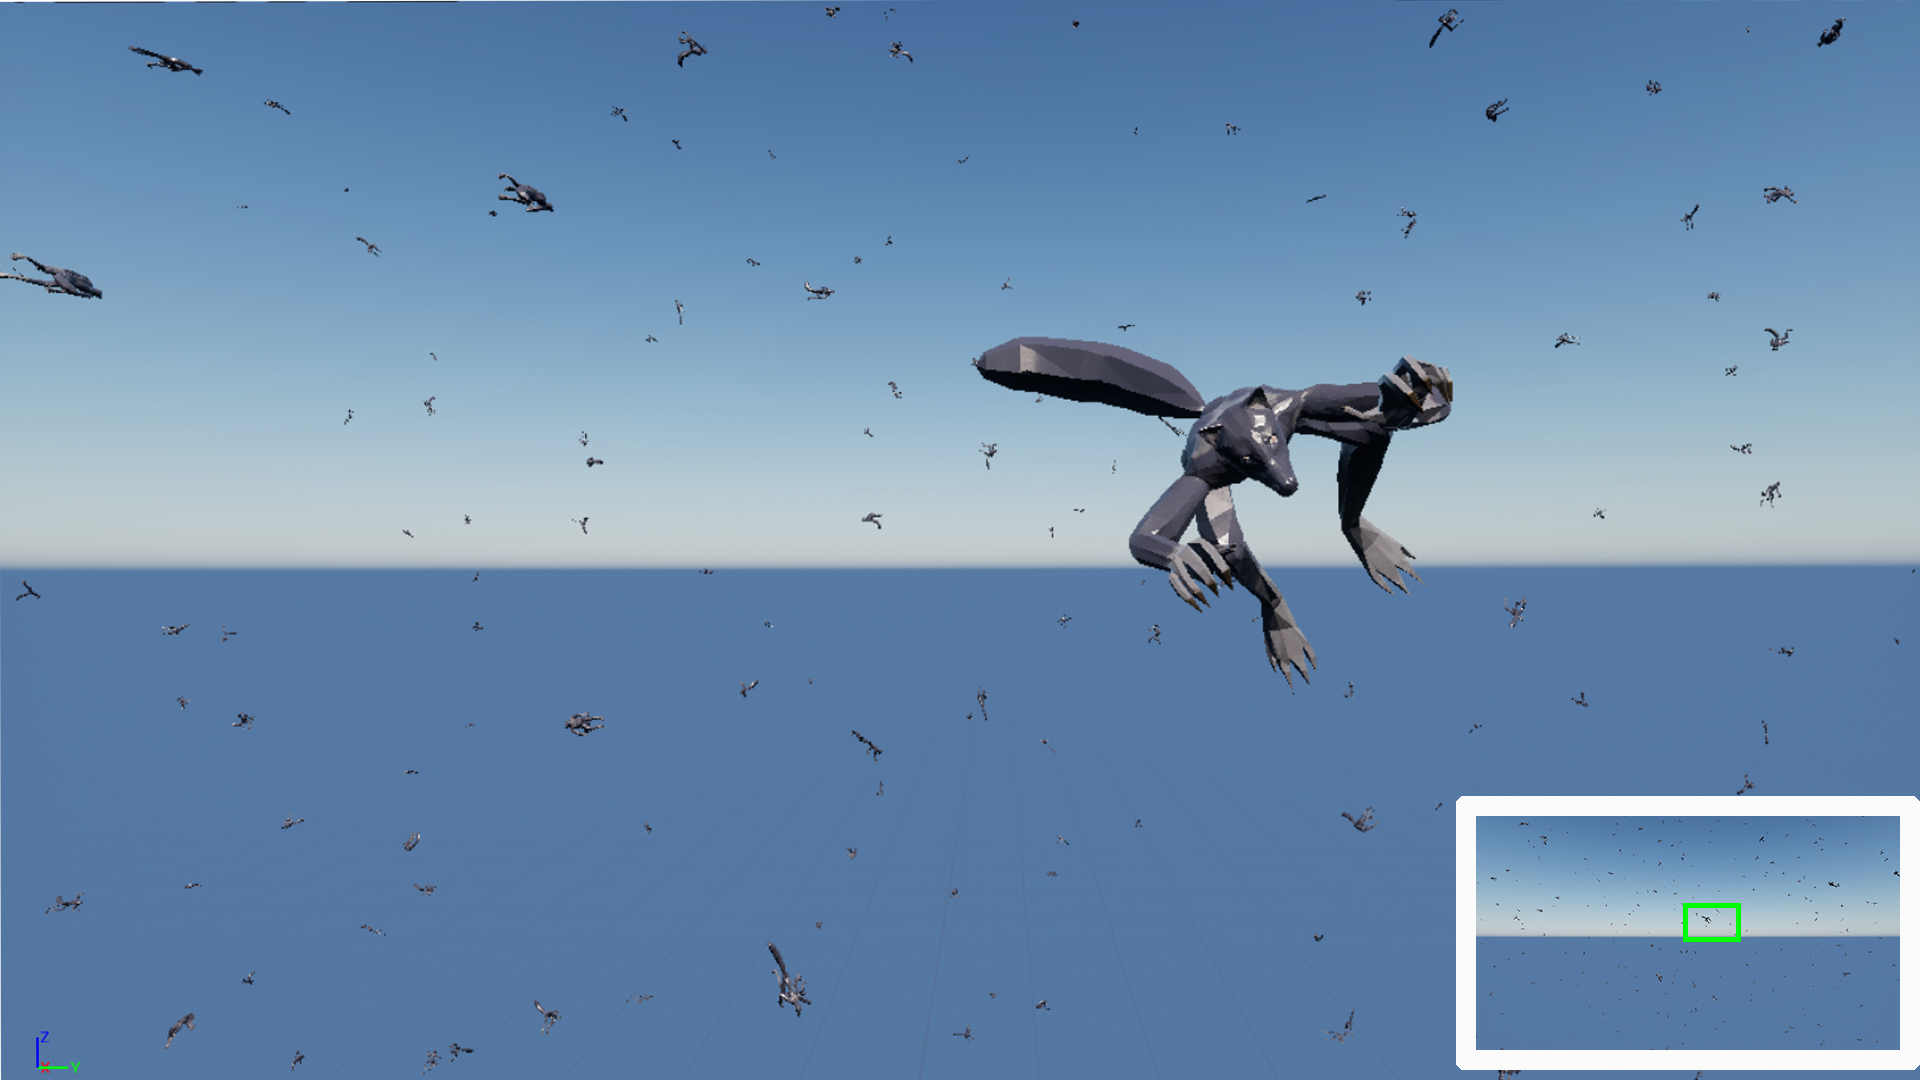
\includegraphics[width=16cm]{figures/UnrealLupa.png}
    \caption{Wygląd testu silnika Unreal Engine w losowym momencie}
    \label{Fig:TESTUnrealScreenLUPA}
\end{figure}     


\clearpage
\section{Analiza danych}

W tabeli \ref{Tabela:KomputeryTesty} przedstawiono 7 komputerów, które zostały
użyte do przetestowania wydajności silników. Wśród komputerów 6 jest komputerami
stacjonarnymi,\\a jeden to laptop. Wśród używanych komputerów pojawiają się różne
karty graficzne. Komputerem z najwolniejszą kartą graficzną jest PC6, a z
najszybszą PC4. Komputerami z największym taktowaniem pamięci RAM są PC3
i PC2. Najwolniejszą pamięć RAM posiada PC6. Najwolniejszy procesor posiada PC7.
Najszybsze procesory znajduje się w komputerze PC2. PC3 zawiera najnowszy model
procesora, ale jest to wersja dedykowana dla laptopów, przez co jest wolniejszy.
Tylko PC2 używał systemu Windows 11, a reszta używała systemu Windows 10.  

\begin{table}[ht]
    \caption{Komputery użyte do testów}
    \centering		
        \begin{tabular}{|c|c|c|c|c|c|}	
            \hline
            LP & Typ jednostki & Procesor & Pamięć RAM & Karta Graficzna  \\
            \hline
            PC1 & K. stacjonarny & Ryzen 5 3600 & 16GB 3200MHz & GeForce RTX 2070 8GB\\
            \hline
            PC2 & K. stacjonarny & Ryzen 5 5600 & 32GB 4800MHz & GeForce RTX 4060 8GB  \\
            \hline
            PC3 & Laptop & Ryzen 5 6600H & 16GB 4800MHz & GeForce RTX 3050 4GB  \\
            \hline
            PC4 & K. stacjonarny & Ryzen 5 3600 & 16GB 3333MHz & Radeon RX6800 16GB \\
            \hline
            PC5 & K. stacjonarny & Ryzen 5 3600X & 16GB 2133MHz & Radeon RX 580 8GB\\
            \hline
            PC6 & K. stacjonarny & i7-3770K & 16GB 1333MHz & GeForce GTX 1050 Ti 4GB \\
            \hline
            PC7 & K. stacjonarny & i5 4460 & 16GB 1600MHz & Radeon RX6600 8GB \\
            \hline

        \end{tabular}	
    \label{Tabela:KomputeryTesty}
\end{table}	




W tabelach \ref{Tabela:StatystykiUnity1} i \ref{Tabela:StatystykiUnity2}
przedstawiono dane statystyczne stworzone na podstawie zebranych danych dla
silnika unity. Minimalna liczba klatek mieściła się w przedziale <3.00, 5.52>. W
przypadkach 4 komputerów minimalna liczba FPS wynosiła 3.00 co może się wiązać z
działaniem silnika. Maksymalna liczba FPS wynosiła 50.00 dla wszystkich
komputerów poza PC7, dla którego wyniosła 60.06. Te wyniki zostały odnotowane
podczas rozstawiania modeli w silniku. Średnia liczba klatek mieściła się\\w
przedziale <17.77, 34.25>. Średnia liczba klatek była najniższa w komputerze z
najsłabszym procesorem, a najwyższa w przypadku PC4. Odchylenie standardowe
liczby klatek na sekundę mieściło się w przedziale od <3.15, 4.75>, co świadczy
o sporym odchyleniu od wartości średniej. Najgorsze 1\% i 0.1\% klatek
na sekundę odbiega od wartości średniej o ponad 10 FPS w prawie wszystkich
przypadkach co świadczy\\o dużych fluktuacjach w prędkości wyświetlanego obrazu.
Wymagany minimalny czas pracy procesora nie przekraczał 42 milisekund.
Największy maksymalny czas pracy procesora został odnotowany w PC4, który
posiadał najniższy minimalny czas pracy.  Średnia czasu pracy procesora mieściła
się w przedziale <29.29, 52.59>. Silnik Unity używał średnio ok 770MB pamięci
RAM i wartość średnia była podobna dla wszystkich komputerów. Wartości
maksymalne nie odbiegały znacząco od wartości średnich. Minimalne użycie pamięci
RAM oscylowało wokół 700MB i najwięcej używał komputer z najsłabszym procesorem
PC7. W użyciu czasu karty graficznej można zauważyć duże różnice między
jednostkami, które są zależne mocy kart graficznych. Największe wartości
minimalnego, maksymalnego oraz średniego czasu użycia zostały odnotowane dla
komputera PC6. Najniższy średni i maksymalny czas pracy został odnotowany dla
komputera PC4, a najniższy średni czas pracy został odnotowany dla komputera
PC2, co świadczy o tym, że komputer z szybszym procesorem średnio używał mniej
czasu karty graficznej, niż komputer z szybszą kartą graficzną. Ostatnimi
wartościami w tabelach są minimalne, maksymalne i średnie użycie pamięci VRAM
karty graficznej.\\W teście średnio używano ok 2400MB pamięci VRAM z małymi
odchyleniami\\w zależności od komputera i podobne zjawisko zachodzi w przypadku
wartości maksymalnych, które nie odbiegają znacząco od wartości średnich.
Minimalne użycie pamięci VRAM jest podobne dla wszystkich komputerów poza PC7,
który używał ok. 700MB pamięci więcej. 
Podsumowując użycie zasobów różnych komputerów można dojść do następujących
wniosków:
\begin{itemize}
\item Test unity działał lepiej na PC4 osiągając średnio 34.25 klatek na
sekundę\\z odchyleniem standardowym  na poziomie 4.15. Najgorszy 1\% i 0.1\%
różni się od siebie w znaczący sposób, co świadczy od dużych fluktuacjach; 

\item Laptop używany w teście nie odbiegał znacząco od komputerów stacjonarnych
w wynikach poza maksymalnym użyciem czasu procesora, który wyniósł 730 ms, co
było najwyższym uzyskanym wynikiem; 

\item Silnik unity wymaga więcej mocy procesora niż karty graficznej, o czym
świadczy różnica między użyciem karty graficznej i procesora, ale najlepszy
wynik został zanotowany na komputerze z 4 najlepszym procesorem i najlepszą
kartą graficzną wśród komputerów; 

\item Unity używa ok.770MB pamięci RAM i ok 2400MB pamięci VRAM niezależnie od
mocy obliczeniowej procesora i karty graficznej. Wartości maksymalne są mocno
zbliżone do wartości średnich. 
\end{itemize}

\begin{table}[h]
    \caption{Dane statystyczne zebrane z komputerów w Unity cz.1}
    \centering		
        \begin{tabular}{|p{1cm}|p{1cm}|p{1cm}|p{1cm}|p{1cm}|p{1cm}|p{1cm}|p{1cm}|p{1,5cm}|p{1cm}|}	
            \hline
            LP & Min FPS & Max FPS & Avg FPS & Std FPS & Worst 1\% & Worst 0.1\% & Min CPU (ms) & Max CPU (ms)  & Avg CPU (ms) \\
            \hline
            PC1 & 5.33 & 50.00 & 31.34 & 4.29 & 20.68 & 19.60 & 24.64 & 72.70 & 31.19 \\
            \hline
            PC 2 & 5.52 & 50.00 & 33.48 & 4.55 & 22.22 & 18.54 & 22.88 & 57.00 & 29.29 \\
            \hline
            PC 3 & 5.26 & 50.00 & 31.09 & 4.75 & 16.68 & 14.71 & 24.56 & 64.38 & 32.07 \\
            \hline
            PC 4 & 3.00 & 50.00 & 34.25 & 4.15 & 19.22 & 5.24 & 18.49 & 730.92 & 30.66 \\
            \hline
            PC 5 & 3.00 & 50.00 & 22.53 & 3.60 & 14.10 & 10.97 & 32.02 & 97.24 & 42.73 \\
            \hline
            PC 6 & 3.00 & 50.00 & 20.47 & 3.21 & 9.55 & 8.33 & 36.41 & 144.98 & 47.93 \\
            \hline
            PC 7 & 3.00 & 60.06 & 17.77 & 3.15 & 11.98 & 10.00 & 41.41 & 296.63 & 52.59 \\
            \hline
        \end{tabular}	
    \label{Tabela:StatystykiUnity1}
\end{table}	

\begin{table}[h]
        \caption{Dane statystyczne zebrane z komputerów w Unity cz.2}
        \centering		
        \begin{tabular}{|p{1cm}|p{1,3cm}|p{1,3cm}|p{1,3cm}|p{1cm}|p{1cm}|p{1cm}|p{1,5cm}|p{1,5cm}|p{1,5cm}|}	
            \hline
            LP & Min RAM Usage (MB) & Max RAM Usage (MB) & Avg RAM Usage (MB) & Min GPU (ms) & Max GPU (ms)  & Avg GPU (ms) & Min VRAMUsage (MB) & Max VRAMUsage (MB) & Avg VRAMUsage (MB) \\
            \hline
            PC1 & 698.84 & 773.10 & 772.16 & 2.37 & 46.20 & 15.12 & 302.44 & 2496.94 & 2452.35 \\
            \hline
            PC2 & 698.84 & 777.10 & 776.03 & 1.78 & 40.31 & 13.71 & 265.52 & 2460.02 & 2415.44 \\
            \hline
            PC3 & 698.84 & 777.10 & 776.03 & 2.91 & 60.89 & 20.58 & 265.52 & 2460.02 & 2415.42 \\
            \hline
            PC4 & 698.84 & 779.10 & 775.41 & 0.05 & 32.11 & 16.32 & 265.52 & 2472.02 & 2417.40 \\
            \hline
            PC5 & 698.84 & 773.10 & 772.21 & 0.79 & 68.11 & 17.85 & 265.52 & 2460.02 & 2415.30 \\
            \hline
            PC6 & 697.59 & 775.85 & 774.72 & 3.53 & 100.53 & 33.20 & 265.52 & 2460.02 & 2415.37 \\
            \hline
            PC7 & 715.47 & 770.60 & 770.45 & 2.11 & 97.06 & 25.22 & 997.93 & 2565.50 & 2533.38 \\
            \hline

            \hline
    
        \end{tabular}	
    \label{Tabela:StatystykiUnity2}
\end{table}	


Tabele \ref{Tabela:StatystykiUnreal1} i \ref{Tabela:StatystykiUnreal2}
przedstawiają statystyki opracowane na bazie danych zebranych podczas testów
silnika Unreal Engine przeprowadzonych na komputerach przedstawionych w
tabeli\ref{Tabela:KomputeryTesty}. Minimalna liczba klatek na sekundę jest niska
dla wszystkich jednostek i nie przekracza wartości 0.77. Najwyższe wartości
średnie i maksymalne klatek w teście zostały osiągnięte przez PC1, co świadczy o
tym, że na szybkość generowania klatek mają wpływ inne czynniki niż moc
obliczeniowa karty graficznej\\i procesora. Istnieje możliwość, że PC2 osiągną
słabszy wynik ze względu na system operacyjny. Nieznacznie niższy wynik średniej
ilości FPS osiągną PC4 z niższą wartością odchylenia standardowego. Najgorszy
wynik uzyskał PC6, z najgorszymi podzespołami. Odchylenie standardowe liczby
klatek jest zależne od podzespołów komputera, ale największą wartość osiągną
PC3. Wartość najgorszego 1\% i 0.1\% jest mniejsza od wartości średniej
odpowiednio w przedziale (3,5) i (4,10) i jest zależne od mocy obliczeniowej
komputera. Najniższa wartość najgorszego 0.1\% klatek został odnotowany dla PC4,
co świadczy o rzadkich, ale większych spadkach stabilności wyświetlania obrazu.
Użycie procesora nie jest zależne od jego mocy, ponieważ komputer z
najwolniejszym procesorem średnie użycie czasu pracy procesora na poziomie
zbliżonym do komputerów\\z szybszymi procesorami. Najdłużej średnio procesor
pracował w komputerze z najwolniejszą kartą graficzną, ale najdłuższy czas pracy
procesora w klatce został zanotowany dla komputera PC5. Minimalne użycie czasu
pracy procesora nie przekroczyło wartości 8ms i w 3 przypadkach było mniejsze
niż 0.5ms. Użycie pamięci RAM było zbliżone dla wszystkich komputerów.
Maksymalnie test używał 1515MB pamięci na komputerze PC5. Ten sam komputer
posiadał najwyższe średnie użycie pamięci RAM, które odbiegało od drugiego
najwyższego wyniku o ok. 40 MB i wynosiło 1303. Najmniej tej pamięci używał PC2.
Te wyniki sugerują, że użycie RAM’u jest zależne od podzespołów komputera. W
przypadku użycia czasu pracy karty graficznej można zauważyć, czas pracy tego
podzespołu jest zależny od jego mocy. Karta graficzna PC4 pracowała najkrócej, a
PC5 najdłużej. Minimalny czas pracy karty graficznej wyniósł dla wszystkich
komputerów 0ms i było to podczas ładowania poziomu. W przypadku pamięci VRAM
karty graficznej jej średnie i maksymalne zużycie jest różne dla wszystkich
jednostek i oscyluje odpowiednio między wartościami <756,1375>MB i <1024,
1932>MB. Minimalne użycie pamięci VRAM było równe dla wszystkich komputerów i
wynosiło 0.02MB. Ta wartość została odnotowana w czasie ładowania poziomu. 


\begin{table}[H]
    \caption{Dane statystyczne zebrane z komputerów w Unreal Engine cz.1}
    \centering		
        \begin{tabular}{|p{1cm}|p{1cm}|p{1cm}|p{1cm}|p{1cm}|p{1cm}|p{1cm}|p{1cm}|p{1,5cm}|p{1cm}|}	
            \hline
            LP & Min FPS & Max FPS & Avg FPS & Std FPS & Worst 1\% & Worst 0.1\% & Min CPU (ms) & Max CPU (ms)  & Avg CPU (ms) \\
            \hline
            PC1 &0.72 & 17.62 & 14.75 & 1.13 & 11.29 & 10.65 & 1.85 & 76.75 & 23.77  \\	
            \hline
            PC2 & 0.77 & 12.30 & 10.26 & 0.57 & 8.80 & 7.89 & 7.99 & 65.53 & 31.30 \\
            \hline
            PC3 & 0.75 & 13.28 & 10.42 & 1.78 & 5.55 & 5.07 & 0.10 & 166.32 & 30.74  \\
            \hline
            PC4 & 0.62 & 16.69 & 14.24 & 0.98 & 10.99 & 8.55 & 0.29 & 77.37 & 23.13  \\
            \hline
            PC5 & 0.69 & 15.78 & 12.39 & 1.30 & 9.15 & 2.55 & 3.15 & 248.33 & 27.82  \\
            \hline
            PC6 & 0.60 & 8.75 & 6.96 & 1.34 & 3.57 & 3.28 & 3.00 & 189.06 & 51.07  \\
            \hline
            PC7 & 0.26 & 14.64 & 10.49 & 1.34 & 7.41 & 7.11 & 0.21 & 103.86 & 29.82 \\
            \hline

        \end{tabular}	
    \label{Tabela:StatystykiUnreal1}
    \end{table}	

Po analizie danych statystycznych na temat użycia zasobów przez silnik Unreal
Enigne można dojść do następujących wniosków:
\begin{itemize}
\item Na działanie programów w silniku Unreal Engine mogą mieć wpływ inne
czynniki niż moc obliczeniowa karty graficznej czy procesora;
\item Stabilność generowania klatek jest zależna od mocy procesora i karty
graficznej;
\item Unreal wykorzystuje w teście więcej mocy obliczeniowej karty graficznej
niż mocy procesora;
\item Ilość używanej pamięci RAM i VRAM przez program nie jest równa dla
wszystkich komputerów na których wykonano testy. Różnice wyniosły 400MB w
przypadku pamięci RAM i ok. 900MB w przypadku VRAM’u;
\item W trakcie ładowania poziomu silnik nie wykorzystuje karty graficznej;
\item W przypadku komputera z systemem Windows 11 został odnotowany słabszy
wynik, co może być powiązane z różnicami między systemami Windows 10\\i Windows
11. 

\end{itemize}
\begin{table}[H]
    \caption{Dane statystyczne zebrane z komputerów w Unreal Engine cz.2}
    \centering		
        \begin{tabular}{|p{1cm}|p{1,1cm}|p{1,4cm}|p{1,4cm}|p{1cm}|p{1,3cm}|p{1cm}|p{1cm}|p{1,5cm}|p{1,5cm}|}	
            \hline
            LP & Min RAMUsage (MB) & Max RAM Usage (MB) & Avg RAM Usage (MB) & Min GPU (ms) & Max GPU (ms)  & Avg GPU (ms) & Min VRAM Usage (MB) & Max VRAM Usage (MB) & Avg VRAM Usage (MB) \\
            \hline
            PC1 & 891.84 & 1192.42 & 1147.32 & 0.00 & 495.69 & 41.44 & 0.02 & 1376.75 & 1347.87 \\
            \hline
            PC2 & 895.72 & 1107.62 & 1059.57 & 0.00 & 275.53 & 30.45 & 0.02 & 1042.42 & 756.09 \\
            \hline
            PC3 & 967.32 & 1270.13 & 1219.99 & 0.00 & 916.77 & 77.82 & 0.02 & 1552.02 & 993.64 \\
            \hline
            PC4 & 914.39 & 1339.31 & 1159.13 & 0.00 & 179.04 & 14.95 & 0.02 & 1605.20 & 1373.53 \\
            \hline
            PC5 & 868.34 & 1432.96 & 1264.48 & 0.00 & 511.32 & 48.57 & 0.02 & 1932.48 & 1343.09 \\
            \hline
            PC6 & 870.37 & 1515.11 & 1303.42 & 0.00 & 1408.78 & 127.18 & 0.02 & 1733.08 & 1375.39 \\
            \hline
            PC7 & 820.81 & 1175.81 & 1129.66 & 0.00 & 257.55 & 22.68 & 0.00 & 1752.53 & 906.55 \\
            \hline
            \hline

        \end{tabular}	
\label{Tabela:StatystykiUnreal2}
\end{table}	


Rysunki
\ref{Fig:PC1Tests}, \ref{Fig:PC2Tests}, \ref{Fig:PC3Tests}, \ref{Fig:PC4Tests},
\ref{Fig:PC5Tests}, \ref{Fig:PC6Tests}, \ref{Fig:PC7Tests} przedstawiają wykresy
klatek na sekundę od czasu przebiegu testów dla różnych komputerów. Na wykresach
kolorem niebieskim oznaczono dane zebrane w czasie testu silnika unity, a na
pomarańczowo dla silnika Unreal Engine. Wykresy zostały ograniczone do 1800
sekund trwania testu. Czas trwania testów nie był stały. W przypadku Unity dla
większości przypadków test trwał ok. 30 minut, poza jednym przypadkiem PC4, na
którym test trwał ok. 50 minut. Dla silnika Unreal Engine długość testu zależała
od średniej liczby klatek. W najgorszym przypadku test trwał ok. 2 godziny.
Zadziałał tutaj mechanizm, który spowalnia upływ czasy w świecie silnika i
spowolnienie jest zależne od szybkości wyświetlania obrazu. 

Wszystkie wykresy dla testów silnika Unity posiadają dolinę w podobnym miescu
trwania testu, która znajduje się parędziesiąt sekund od zaczęcia testu i trwa
do 200 sekund. Pod koniec trwania testu zachodzi podobne zjawisko. Ze względu na
zaistnienie zjawiska w testach na różnych komputerach oraz ze względu na fakt,
że występują one w tym podobnym miejscu w czasie, to jest to cecha silnika
Unity. W pierwszych sekundach wykresy mają wartość 50 lub 60 klatek na sekundę.
Na wykresach najmniejsze fluktuacje zachodzą na wykresie \ref{Fig:PC6Tests}.
Dziwne zachowanie można zaobserwować na wykresie \ref{Fig:PC7Tests}, gdzie
wykres ma wartość ok. 30 klatek na sekundę i są to pojedyncze skoki. Największe
fluktuacje na wykresie znajdują się na wykresie \ref{Fig:PC4Tests}. Poza tym na
wszystkich wykresach można zaobserwować spadki, które wynoszą ponad 10 klatek,\\a
na niektórych spadki wynoszą nawet 20 klatek na sekundę. 

Wszystkie wykresy dla silnika Unreal Engine posiadają dolinę kilkadziesiąt
sekund od rozpoczęcia testu, jednak nie jest ona tak głęboka jak w przypadku
testów wykonanych na silniku Unity. Dolina ta jest głęboka na ok. (2,5) FPS.
Jedynymi wyjątkami są PC6 \ref{Fig:PC6Tests} i PC3 \ref{Fig:PC3Tests}. Długość
doliny jest zależna od sprzętu na którym został wykonany test. Początek wykresu
zaczyna się wartością bliską 0. Fluktuacje na wykresach są niewielkie i poza
nielicznymi przypadkami nie ma większych odchyleń od średniej. Największe
fluktuacje zachodziły dla PC4 \ref{Fig:PC4Tests} Test silnika Unreal trwał
dłużej.

Liczba FPS w teście silnika Unity była znacząco wyższa niż silnika Unreal
Enigne, ale też z dużo większymi fluktuacjami. Silnik Unreal Engine był bardzo
stabilny z niewielkimi odchyleniami do średniej. W wykresach obu testów ukazały
się pewne błędu lub niedociągnięcia silników w początkowych fazach testów.
Występowanie dolin w podobnych miejscach testu pokazuje podobieństwo w
silnikach. Silniki w podobnym czasie testu natrafiają na problematyczną część,
która sprawia, że wymagana jest większa liczba obliczeń. W silniku Unreal doliny
zostały rozciągnięte przez wspomniany mechanizm, ale były one bardziej płaskie. 



\begin{figure}[h]
    \centering
    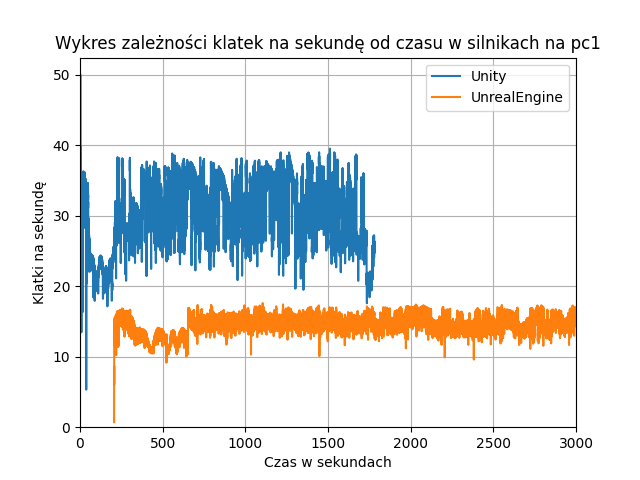
\includegraphics[width=16cm]{figures/FPSPlots/pc1searchedDataName.png}
    \caption{Liczba klatek na sekundę generowana dla testów przeprowadzonych na PC1}
    \label{Fig:PC1Tests}
\end{figure}        

\begin{figure}[ht]
    \centering
    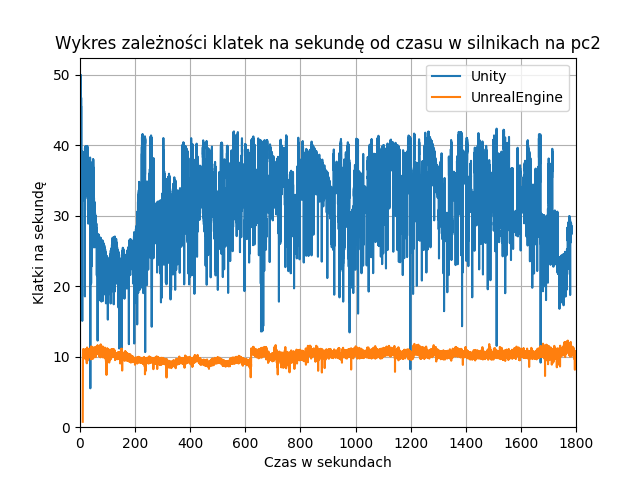
\includegraphics[width=16cm]{figures/FPSPlots/pc2searchedDataName.png}
    \caption{Liczba klatek na sekundę generowana dla testów przeprowadzonych na PC2}
    \label{Fig:PC2Tests}
\end{figure}        

\begin{figure}[ht]
    \centering
    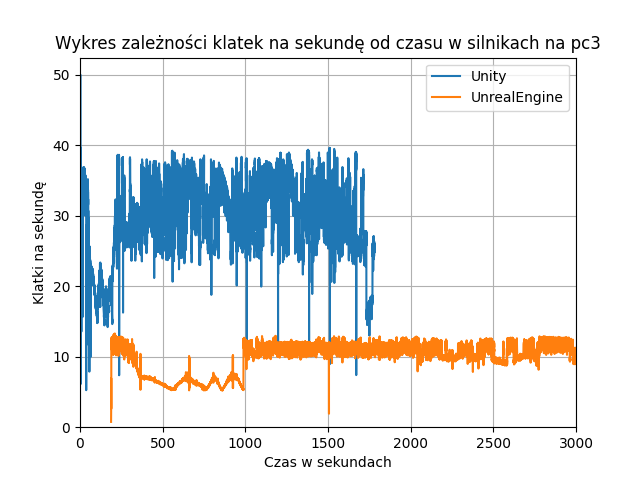
\includegraphics[width=16cm]{figures/FPSPlots/pc3searchedDataName.png}
    \caption{Liczba klatek na sekundę generowana dla testów przeprowadzonych na PC3}
    \label{Fig:PC3Tests}
\end{figure}        

\begin{figure}[ht]
    \centering
    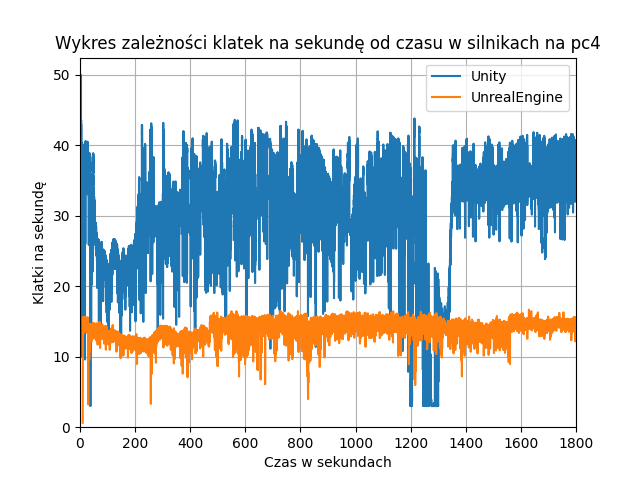
\includegraphics[width=16cm]{figures/FPSPlots/pc4searchedDataName.png}
    \caption{Liczba klatek na sekundę generowana dla testów przeprowadzonych na PC4}
    \label{Fig:PC4Tests}
\end{figure}      

\begin{figure}[ht]
    \centering
    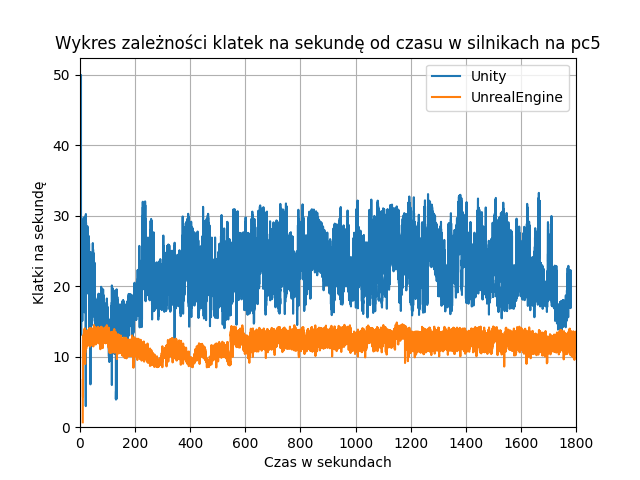
\includegraphics[width=16cm]{figures/FPSPlots/pc5searchedDataName.png}
    \caption{Liczba klatek na sekundę generowana dla testów przeprowadzonych na PC5}
    \label{Fig:PC5Tests}
\end{figure}    
\begin{figure}[ht]
    \centering
    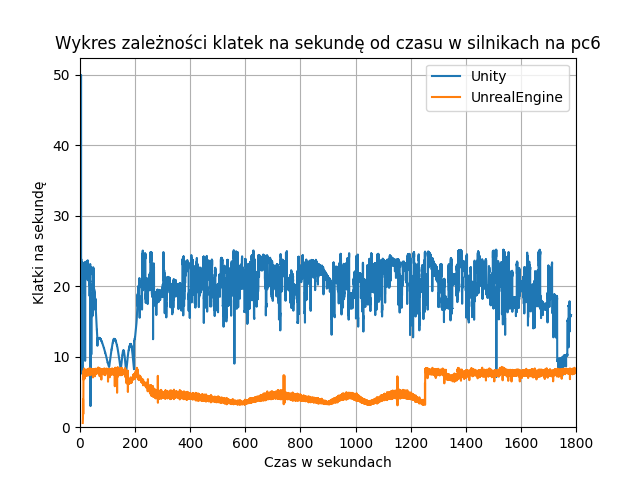
\includegraphics[width=16cm]{figures/FPSPlots/pc6searchedDataName.png}
    \caption{Liczba klatek na sekundę generowana dla testów przeprowadzonych na PC6}
    \label{Fig:PC6Tests}
\end{figure}      

\begin{figure}[ht]
    \centering
    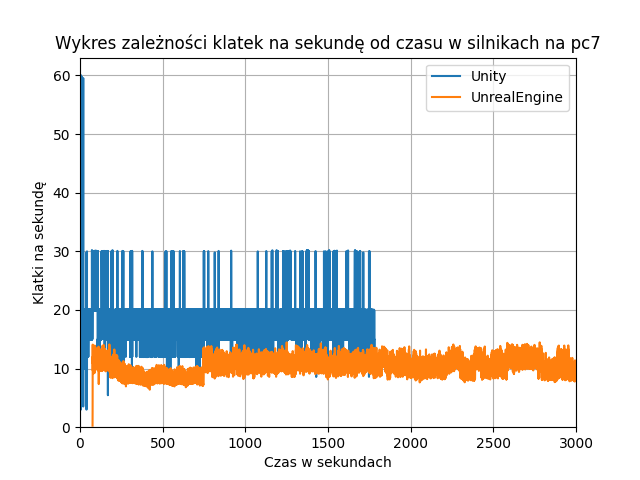
\includegraphics[width=16cm]{figures/FPSPlots/pc7searchedDataName.png}
    \caption{Liczba klatek na sekundę generowana dla testów przeprowadzonych na PC7}
    \label{Fig:PC7Tests}
\end{figure}    





\clearpage


\section{Podsumowanie i wnioski}

Silniki graficzne wywodząc się z środowiska gier komputerowych i branży filmowej
ugruntowały swoją pozycję w świecie. Gry i filmy stały się ważnym elementem
kultury już w latach 2000, a wraz z biegiem czasu coraz bardziej zyskiwały na
znaczeniu.  W dzisiejszych czasach największe branża gier i filmów korzystają z
różnych silników graficznych zagnieżdżonych w różnych programach. Silniki
graficzne zostały znacząco rozwinięte i pozwalają na tworzenie niezwykle
realistycznych efektów wizualnych.

Silniku Unity i Unreal Engine są jednymi z najbardziej popularniejszych
komercyjnych silników graficznych używanych w produkcji gier. Oba silniki
posiadają swoje wady i zalety. Unity jest silnikiem prostym i przez użycie
języka C\# do tworzenia skryptów bardziej przystępny dla początkujących twórców
gier. Unreal Enigne używając kombinacji blueprint’ów i języka C$++$ pozwala na
płynne tworzenie i optymalizowanie funkcjonalności gier. Oba silniki znacząco
różnią się pod względem podstawowej infrastruktury oraz skalowalności silnika.
Silnik Unity pozwala na stworzenie demonstracyjnej wersji gry bardzo szybko, ale
wymaga więcej pracy i wiedzy przy ambitnych projektach. Unreal Enigne wymaga
sporo pracy w początkowej fazie tworzenia gry, ale wraz z jej rozwojem wbudowane
elementy przyśpieszają proces. 

Przeprowadzone testy zostały ograniczone do jednej części silnika graficznego
jakim jest rendering dynamicznie rozstawionych obiektów. Oba silniki były
testowane\\w swojej podstawowej formie. W silniku Unreal Engine został wyłączony
system Lumen, który jest zaawansowaną techniką oświetlenia, która jest
wielokrotnie bardziej skomplikowana niż model oświetlenia silnika Unity. Test
polegał na rozstawieniu 4000 tysięcy modeli wraz z animacjami w przestrzeni i
przejściu przez kamerę pewnej wcześniej ustalonej ścieżki. Rozstawienie modeli
zostało wcześniej ustalone i zapisane\\w pliku. Programy musiały odczytać
rozstawienie i rozstawić modele. Dane były zbierane przez narzędzia wbudowane w
silniki i zapisywane przez skrypt silnika. Programy testowe zbudowane z silników
zostały uruchomione na 7 komputerach z różną specyfikacją. Jako obiekty zostały
użyte modele wraz z zestawem animacji szkieletowych. 

Wyniki testów można przedstawić następująco:
\begin{itemize}
\item Silnik Unity używał maksymalnie ok. 770MB pamięci RAM i ok. 2500MB pamięci
karty graficznej oraz te wartości minimalnie się zmieniały dla komputerów.
Unreal Enigne używał więcej pamięci RAM o ok. 400MB i mniej pamięci VRAM o ok.
900MB i ilość używanej pamięci była zależna od specyfikacji komputera; 

\item Unity wymaga więcej mocy obliczeniowej procesora, ale moc karty graficznej
również ma wpływ na szybkość generowania klatek;

\item Generacja obrazu była stabilniejsza przy pomocy Unlreal Engine’a, niż w
przypadku Unity. Testy silnika Unreal wykazały mniejszą ilość fluktuacji oraz mniejszą ich siłę. Silniki miały problem w podobnym momencie testów, co miało
swoje odzwierciedlenie w wykresach liczby klatek od czasu;


\item Unreal Engine wymaga większej mocy obliczeniowej karty graficznej, ale moc
procesora również ma pewien wpływ na przebieg testu;

\item System Windows 11 może mieć większy wpływ na przebieg testu niż system
Windows 10, ale należy to sprawdzić na komputerach z takimi samymi podzespołami;

\item Silniki Unreal Enigne nie wykorzystuje karty graficznej podczas ładowania
poziomu i rozstawiania modeli. Takie zjawisko nie zachodzi przy działaniu
silnika Unity;

\item Czas trwania testów w silniku Unreal był dłuższy i był zależny od mocy
obliczeniowej komputera, w najgorszym przypadku test trwał ponad 2 godziny.\\W
przypadku silnika Unity test trwał podobną ilość czasu równą ok. 30 minut poza
jednym przypadkiem, gdzie test skończył się po 50 minutach. 


\end{itemize} 
Autor za wkład własny uważa:
\begin{itemize}
\item Opis infrastruktury silników Unity i Unreal Engine;
\item Wskazanie różnic między silnikami;
\item Opisanie zasad testów;
\item Stworzenie testów na obu silnikach;
\item Przeprowadzenie testów;
\item Analiza i wyciągnięcie wniosków na bazie zebranych danych;
\end{itemize}


\clearpage

\section*{Załączniki}
\addcontentsline{toc}{section}{Załączniki}
\begin{itemize}
    \item  pliki projektów użytych do zbudowania programów testowych
    \item zebrane dane wraz ze specyfikacją używanych komputerów
    
\end{itemize}


\clearpage

\addcontentsline{toc}{section}{Literatura}

\begin{thebibliography}{4}
\bibitem{GameEngineArchitecture} Jason Gregory: Game Engine Architecture, CRC Press 2019
\bibitem{GameDevelpomenPhysics} David M. Bourg, Bryan Bywalec: Physics for Game Development, O\'Reilly 2013

\bibitem{Blender:EEVEE} \url{https://docs.blender.org/manual/en/latest/render/eevee/introduction.html} Dostęp \today
\bibitem{Blender:Cycles} \url{https://docs.blender.org/manual/en/2.80/render/cycles/introduction.html} Dostęp \today
\bibitem{Blender:Workbench} \url{https://docs.blender.org/manual/en/3.3/render/workbench/introduction.html} Dostęp \today



\bibitem{Unity:Documentatnion} \url{https://docs.unity.com/} Dostęp \today
\bibitem{Unity:DonSaveOnLoad} \url{https://docs.unity3d.com/ScriptReference/Object.DontDestroyOnLoad.html} Dostęp \today
\bibitem{Unity:Scena} \url{https://docs.unity3d.com/Manual/CreatingScenes.html} Dostęp \today
\bibitem{Unity:Obiekt} \url{https://docs.unity3d.com/Manual/GameObjects.html} Dostęp \today

\bibitem{Unity:Awake} \url{https://docs.unity3d.com/ScriptReference/MonoBehaviour.Awake.html} Dostęp \today
\bibitem{Unity:StateChangeExit} \url{https://docs.unity3d.com/ScriptReference/StateMachineBehaviour.OnStateMachineExit.html} Dostęp \today
\bibitem{Unity:StateChangeEnter} \url{https://docs.unity3d.com/ScriptReference/StateMachineBehaviour.OnStateMachineEnter.html} Dostęp \today

\bibitem{Unity:yield} \url{https://docs.unity3d.com/ScriptReference/YieldInstruction.html} Dostęp \today
\bibitem{Unity:ONAnimationIK} \url{https://docs.unity3d.com/ScriptReference/MonoBehaviour.OnAnimatorIK.html} Dostęp \today
\bibitem{Unity:onCurl} \url{https://docs.unity3d.com/ScriptReference/Camera.OnPreCull.html} Dostęp \today
\bibitem{Unity:OnPreRender} \url{https://docs.unity3d.com/ScriptReference/Camera.OnPreRender.html} Dostęp \today
\bibitem{Unity:OnPostRender} \url{https://docs.unity3d.com/ScriptReference/Camera.OnPostRender.html} Dostęp \today

\bibitem{Unity:Flowchart} \url{https://docs.unity3d.com/Manual/ExecutionOrder.html} Dostęp \today

\bibitem{UE:Documentatnion} \url{https://docs.unrealengine.com/4.27/en-US/} Dostęp \today
\bibitem{UnrealEngineArchitecture} \url{https://dev.epicgames.com/documentation/en-us/unreal-engine/gameplay-framework-in-unreal-engine?application_version=5.4} Dostęp: \today

\bibitem{UE:GameInstance} \url{https://docs.unrealengine.com/4.27/en-US/API/Runtime/Engine/Engine/UGameInstance/} Dostęp \today
\bibitem{UE:GameModeState}  \url{https://dev.epicgames.com/documentation/en-us/unreal-engine/game-mode-and-game-state-in-unreal-engine} Dostęp \today
\bibitem{UE:LevelScriptActor}  \url{https://docs.unrealengine.com/4.27/en-US/ProgrammingAndScripting/Blueprints/UserGuide/Types/LevelBlueprint/} Dostęp \today
\bibitem{UE:Controller}  \url{https://docs.unrealengine.com/4.26/en-US/InteractiveExperiences/Framework/Controller/} Dostęp \today
\bibitem{UE:Actor}  \url{https://docs.unrealengine.com/4.27/en-US/ProgrammingAndScripting/ProgrammingWithCPP/UnrealArchitecture/Actors/} Dostęp \today
\bibitem{UE:Pawn}  \url{https://docs.unrealengine.com/4.26/en-US/InteractiveExperiences/Framework/Pawn/} Dostęp \today
\bibitem{UE:Character}  \url{https://docs.unrealengine.com/4.27/en-US/InteractiveExperiences/Framework/Pawn/Character/} Dostęp \today
\bibitem{UE:Component}  \url{https://docs.unrealengine.com/4.27/en-US/ProgrammingAndScripting/ProgrammingWithCPP/UnrealArchitecture/Actors/Components/} Dostęp \today

\bibitem{UE:ActorLifeCycleSource} \url{https://docs.unrealengine.com/4.27/en-US/ProgrammingAndScripting/ProgrammingWithCPP/UnrealArchitecture/Actors/ActorLifecycle/} Dostęp: \today
\bibitem{UE:TickingActor} \url{https://docs.unrealengine.com/4.27/en-US/ProgrammingAndScripting/ProgrammingWithCPP/UnrealArchitecture/Actors/Ticking/} Dostęp \today


\bibitem{SteamSurvey} \url{https://store.steampowered.com/hwsurvey/Steam-Hardware-Software-Survey-Welcome-to-Steam} Dostęp: \today
\bibitem{ModelSource} Kacper Rudź, Sławomir Samolej, Gra platformowa 3D, Politechnika Rzeszowska \url{https://github.com/szczerrzuja/ProjektIn-ynierski-KacperRudz}

\end{thebibliography}

\clearpage

\makesummary

\end{document} 
